\section{Conceptual Foundations of the Institutional Grammar 2.0}
\label{sec:Definitions}

% Header reference level
\clearpairofpagestyles
\chead{Conceptual Foundations of the Institutional Grammar 2.0}
\automark[subsection]{subsection}
\ifoot{\ifootertext}
\ofoot{\ofootertext}
\cfoot{\thepage}


IG 2.0 is premised on a set of syntactic definitions, conceptualizations of institutional statements, and assumptions regarding institutional statements, as well as various forms of nesting (statement-level and component-level nesting). While these definitions, conceptualizations, and assumptions generalize across levels of IG encoding, how they are captured depends on at which level the encoder is working. In this section, we will thus lay out these foundational syntactic definitions, concepts, and assumptions. We start by offering complete definitions of IG components more generally, and then move to defining key institutional statement concepts, including the various notions of nested institutional statements and associated assumptions. We further provide principles and operational guidelines for the identification of statements in as far as they relate to the fundamental concept \begin{emp}Action Situation\end{emp}, namely context characterizations embedded in institutional statements and identification of institutional statement types in the first place. Concluding this section, we organize the coding levels based on involved features, along with providing principal guidelines for the coding process. Note that most concepts in this section are introduced with a pragmatic focus on providing essential foundational understanding to perform the coding of institutional statements. For an extended treatment of the conceptual foundations, refer to \citet{Frantz2022InstitutionalGrammar}.

\subsection{Syntactic Definitions of Institutional Statement Components}
\label{subsec:Syntax}

The IG structure as referred to in this document relies on the elementary syntactic components of regulative and constitutive statements highlighted in Tables \ref{tab:SyntacticElementsRegulative} and \ref{tab:SyntacticElementsConstitutive}. Definitions of these components that hold across IG 2.0 encoding levels are provided alongside each syntactic component.


\begin{table}[h!]
\centering
\begin{tabular}{p{2.3cm} p{14cm}}
\toprule
\textbf{Syntactic Element} & 
\textbf{Definition} \\
\toprule
Attributes & An actor (individual or corporate) that carries out, or is expected to/to not carry out, the action (i.e., Aim) of the statement. The Attributes component may also contain descriptors of the actor. 

The presence of this component is \begin{emp}necessary\end{emp} for any regulative statement.\\
\midrule
Deontic & A prescriptive or permissive operator that defines to what extent the action of an institutional statement is compelled, restrained, or discretionary. 

In institutional statements varying levels of prescriptiveness or strength thereof are represented with different terms or language that situate along a continuum.

The presence of this component is \begin{emp}optional\end{emp} for regulative statements.\\
\midrule
Aim & The goal or action of the statement assigned to the statement Attribute. 

The presence of this component is \begin{emp}necessary\end{emp} for any regulative statement.\\
\midrule
Object & The inanimate or animate part of an institutional statement that is the receiver of the action captured in the Aim. Objects can be of \begin{emp}direct\end{emp} or \begin{emp}indirect\end{emp} nature. Indirect objects are objects that are affected or targeted by the application of the Aim to direct objects. Objects can both be real-world entities, or abstract ones (e.g., beliefs, concepts, facts, procedures). Abstract objects here further include complex constructs, such as conditions/processes that the responsible actor is or will be acting upon. Such complex objects  can potentially take the structural form of institutional statements themselves. 

The presence of this component is \begin{emp}optional\end{emp} for regulative statements.\\
\midrule
Context & The context component instantiates settings in which the focal action of a statement applies, or qualifies the action indicated in an institutional statement. The former type of Context is referred to as an \begin{emp}``Activation Condition''\end{emp}. The latter type of Context is referred to as an \begin{emp}``Execution Constraint''\end{emp}. Both can occur in a given institutional statement, including multiples of either type. 

The presence of this component is \begin{emp}necessary\end{emp} for any regulative statement, but can be implied (as with the original institutional grammar). Where no explicit Activation Condition is specified, the context clause is by default ``under all conditions''. Where no explicit Execution Constraints are specified, the context clause is by default ``no constraints''. 

It is important to note that \begin{emp}Context\end{emp} in institutional statements reflects the context specific to the coded statement (Statement Context), as opposed to capturing context in the wider sense, making reference to the context of the policy or the domain more generally.\\
\midrule
Or else & A sanctioning provision associated with the action indicated in a particular institutional statement represented in a nested institutional statement (as defined in the following discussion). Where combinations of regulative and constitutive statements are applied (hybrid institutional statements), the consequence can be existential in kind (see \cref{tab:SyntacticElementsConstitutive} and \cref{subsec:ConstitutiveRegulativeHybrids}).

The presence of this component is \begin{emp}optional\end{emp} for regulative statements.\\
\toprule
\end{tabular}
\caption{Definitions of Syntactic Elements for Regulative Statements}
\label{tab:SyntacticElementsRegulative}
\end{table}

\begin{table}[h!]
    \centering
\begin{tabular}{p{2.3cm} p{14cm}}
\toprule
\textbf{Syntactic Element} & 
\textbf{Definition} \\
\toprule
Constituted Entity & The entity being constituted, reconstituted, modified or otherwise directly affected within an institutional statement as characterized by the constitutive function. This can be an entity as relevant in the institutional setting, or the policy itself. 

The presence of this component is \begin{emp}necessary\end{emp} for any constitutive statement.\\
\midrule
Modal & An operator that signals necessity or (im-)possibility of constitution or modification of system features captured in the constitutive function. 

In institutional statements varying levels of necessity or strength thereof are represented with different terms or language that situate along a continuum. 

The presence of this component is \begin{emp}optional\end{emp} for constitutive statements.\\
\midrule
Constitutive Function & An expression that relates the constituted entity and the institutional setting, e.g., by defining, establishing, or modifying the former, including the conferral of status. Where constituting
properties exist, constitutive functions functionally link Constituted Entity and Constituting Properties. 

The presence of this component is \begin{emp}necessary\end{emp} for any constitutive statement.\\
\midrule
Constituting Properties & Constituting Properties parameterize the Constituted Entity via the Constitutive Function, and can both be physical or abstract in kind. Constituting Properties may or may not be present in constitutive statements. 

The presence of this component is \begin{emp}optional\end{emp} for constitutive statements.\\
\midrule
Context & The Context instantiates settings in which the focal Constitutive Function of a statement applies, or qualifies the function indicated in an institutional statement. The former type of Context is referred to as an \begin{emp}``Activation Condition.''\end{emp} The latter type of Context is referred to as an \begin{emp}``Execution Constraint.''\end{emp} Both can occur in a given institutional statement, including multiples of either type. 

The presence of this component is \begin{emp}necessary\end{emp} for any constitutive statement, but can be implied (as with the original institutional grammar). Where no explicit Activation Condition is specified, the context clause is by default ``under all conditions''. Where no explicit Execution Constraints are specified, the context clause is by default ``no constraints''. 

It is important to note that \begin{emp}Context\end{emp} in institutional statements reflects the context specific to the coded statement (Statement Context), as opposed to capturing context in the wider sense, making reference to the context of the policy or the domain more generally.
\\
\midrule
Or else & A consequence characterization associated with the non-fulfilment or -enactment of the Constitutive Function indicated in a separate  institutional statement nesting on the leading institutional statement (as defined in the following discussion). Consequences, as understood in the context of constitutive statements, can be existential in kind (e.g., invalidating policy), as opposed to the non-existential sanctioning provisions on the regulative side. 

The presence of this component is \begin{emp}optional\end{emp} for constitutive statements.\\
\toprule
\end{tabular}
\caption{Definitions of Syntactic Elements for Constitutive Statements}
\label{tab:SyntacticElementsConstitutive}
\end{table}

\newpage

\begin{minipage}{5cm} % Needed to force next page - no other purpose

\end{minipage}

\subsection{Institutional Statements}
\label{subsec:InstitutionalStatementAssumptions}

Capturing both the regulative and constitutive nature of statements, in IG 2.0 \begin{emp}an institutional statement\index{Institutional Statement} describes expected actions for actors within the presence or absence of particular constraints, or parameterizes features of an institutional system.\end{emp}

To accommodate a more comprehensive representation of structure and content, the construction of institutional statements in IG 2.0 requires a differentiated understanding of institutional statements, both in terms of \begin{emp}atomic\end{emp} and \begin{emp}nested institutional statements\end{emp} of various forms. 

\subsubsection{Atomic Institutional Statements}
\label{subsubsec:AtomicInstitutionalStatements}

Before highlighting notions of nested institutional statements, we reiterate the notion of an atomic institutional statement as the elementary form of an institutional statement: an \begin{emp}atomic institutional statement\end{emp}\index{Atomic Institutional Statement} is a statement of regulative or constitutive kind that contains the corresponding necessary components, alongside potential optional components other than the \begin{emp}Or else\end{emp}, and in which none of the components contains multiple values (\begin{emp}component-level combinations\end{emp}) or is otherwise nested (\begin{emp}component-level nesting\end{emp} -- see \cref{subsec:ComponentLevelNesting}). Examples for component-level combinations are multiple attributes or combinations of aims in a given institutional statement. Examples for component-level nesting include context characterizations (with details to be introduced at a later stage) expressed as institutional statements themselves.

Illustrating this concept, the statement \begin{exi}``Organic farmers must commit to organic farming standards''\end{exi} is \begin{emp}atomic\end{emp} in kind. It identifies the following elements:

\begin{itemize}
\item Attributes: Organic farmers
\item Deontic: must
\item Aim: commit to
\item Direct object: organic farming standards
\item (Implied) Context: under all conditions.
\end{itemize}

It does not include an \begin{emp}Or else\end{emp}, and neither of the components contains value combinations.\footnote{Note that a component can contain phrases; however, the terms need to represent a semantic unit in the context of the concerned institutional statement.} 

In contrast, the statement \begin{exi}``Organic farmers must commit to their organic farming standards and accommodate regular reviews of their practices''\end{exi} combines multiple distinctive activities and associated objects, namely \begin{emp}``commit to organic farming standards''\end{emp} and \begin{emp}``accommodate regular reviews of their practices''\end{emp}, as illustrated below by aggregating all phrases by component type (multiple phrases are separated by semicolon). 

\begin{itemize}
\item Attributes: Organic farmers
\item Deontic: must
\item Aim: commit to; accommodate
\item Direct Object:\footnote{The distinction between direct and indirect object is discussed in greater detail at a later stage.} organic farming standards; regular reviews of their practices
\item (Implied) Context: under all conditions.
\end{itemize}

We refer to any such combination of component values as a \begin{emp}component-level combination\end{emp}.

In consequence, this statement is \begin{emp}not atomic\end{emp} in kind.

\subsubsection{Nested Institutional Statements}
\label{subsubsec:NestedInstitutionalStatements}

Motivating the conception of nested institutional statements\index{Nested Institutional Statements} is the pragmatic observation that statements can reflect a linkage or embedding of multiple actors or regulated activities, reflecting complex configurational settings; rules in form are generally not expressed in the atomic form specified above. Lack of specificity of these linkages undermines the coder's ability to comprehensively, and accurately, capture institutional content for versatile downstream analysis.

IG 2.0 accommodates two forms of institutional statement nesting: \begin{emp}horizontal nesting\end{emp} and \begin{emp}vertical nesting\end{emp}. Generally, horizontal nesting\index{Horizontal Nesting} allows for the representation of multiple institutional statements that convey co-occurring or alternative actions, actor or object involvement, i.e., any case in which multiple of the same syntax element occur in an institutional statement. 

Generally, vertical nesting\index{Vertical Nesting} allows for the representation of multiple institutional statements that convey coupled actions that follow from one another in the form of a consequential relationship. It is particularly suited to representing the case of consequentially linked statements in which statement A delineates permitted, required, or forbidden activity (for regulative statements), or is constitutive in kind, and statement B delineates sanctions for non-conformance with statement A. In the IG 2.0 parlance, statement A is considered a ``\begin{emp}monitored statement\index{monitored statement}\end{emp},'' and statement B a ``\begin{emp}consequential statement\index{consequential statement}\end{emp}.'' Horizontal nesting and vertical nesting are described in more detail below.

\sp

\textbf{Horizontal Nesting\index{Horizontal Nesting}}: Horizontal nesting describes a logical combination of two or more statements to capture institutional content comprehensively. Exemplified in narrative form, a horizontally nested statement can combine two or more statements. Borrowing the example introduced earlier (\begin{exi}``Organic farmers must commit to their organic farming standards and accommodate regular reviews of their practices''\end{exi}), horizontal nesting reflects the decomposition of such statement into two logically-combined atomic institutional statements, such as \begin{exa}``Organic farmers must commit to organic farming standards'' \AND ``Organic farmers must accommodate regular reviews of their practices''\end{exa}

Horizontal nesting allows for more complex constructs linking an, in principle, arbitrary number of atomic institutional statements and combinations thereof, such as \begin{exa}(``Organic farmers must commit to organic farming standards'' \AND 

``Organic farmers must accommodate regular reviews of their practices'') \XOR 

(``Organic farmers must \NOT~sell their produce under the organic farming label'').\end{exa}

In this example, we can observe the linkage of three statements, in which two AND-combined statements apply as an alternative (XOR) to a third statement. 

Note the use of parentheses to signal the precedence of individual statements where multiple logical operators are used. 

Possible logical operators for horizontal nesting, or \begin{emp}statement combinations\end{emp}, are \AND~(conjunction), \OR~(inclusive disjunction; colloquially: \begin{hil}AND/OR\end{hil}), or \XOR~(exclusive disjunction; colloquially: \begin{hil}EITHER/OR\end{hil}). Where negation is involved, those can be combined with the operator \NOT~(as highlighted in the previous example). An alternative equivalent representation is \begin{exa}(``Organic farmers must commit to organic farming standards'' \AND 

``Organic farmers must accommodate regular reviews of their practices'') \XOR

\NOT~(``Organic farmers must sell their produce under the organic farming label'').\end{exa}

A common use case in practice is the decomposition of action combinations (e.g., \begin{exi}``\dots establish and maintain \dots''\end{exi}) or multiple actors (e.g., \begin{exi}
``\dots producers or inspectors of the facility \dots''\end{exi}).\footnote{The decomposition of such component-level combinations is discussed as part of the coding guidelines in \cref{sec:CodingGuidelines}, specifically in  \hyperlink{tablink:DecompositionOfComponentLevelCombinationsCoreRegulative}{\cref{tab:CodingIgCoreRegulative}, Item \EntryDecompositionOfComponentLevelCombinations}, as well as \hyperlink{tablink:DecompositionOfComponentLevelCombinationsExtendedRegulative}{the same item in \cref{tab:CodingIgExtendedRegulative}} for regulative statements. \hyperlink{tablink:DecompositionOfComponentLevelCombinationsCoreConstitutive}{\cref{tab:CodingIgCoreConstitutive}, Item \EntryDecompositionOfComponentLevelCombinations} provides guidelines for constitutive statements. General operational guidelines for fine-grained decomposition can be found in \hyperlink{tablink:LogicalRelationshipsAmongStatementComponents}{\cref{tab:CodingIgLogicoRegulative}, Item \EntryLogicalRelationshipsAmongComponents}. Note: All preceding table item references are clickable links.}

\sp

\textbf{Vertical Nesting\index{Vertical Nesting}}: Vertical nesting describes a relationship of two or more statements, in which the leading statement (\begin{emp}monitored statement\end{emp}) describes an action that is regulated by a second statement nested in the Or else component (\begin{emp}consequential statement\end{emp}), rendering the Or else an abstract component backed by a separate institutional statement. More accurately, the Or else does not reflect an IG component, but rather a logical connective that links two institutional statements. In this linkage, the second statement reflects a consequence of violating the instructions captured in the monitored statement. Consequences generally involve some pay-off for non-compliance or compliance.\footnote{Where constitutive statements are involved, consequences can further be existential in kind.} Exemplifying vertical nesting in narrative form, we can write \begin{exa}``Organic farmers must comply with organic farming regulations'', \begin{hil}OR ELSE\end{hil} ``Certifiers must revoke the organic farming certification''.\end{exa} Note that both forms of nesting can be combined, i.e., monitored and consequential statements can embed horizontal nesting. Extending the previous example, we can state (visually supported by indentation to signal the corresponding forms of nesting) 

\begin{exa}(``Organic farmers must comply with organic farming regulations'' \begin{hil}AND\end{hil}\\
\-\hspace{0.43cm}\ ``Organic farmers must accommodate regular review of their practices''), \\
\-\hspace{1.5cm}\ \begin{hil}OR ELSE\end{hil} (``Certifiers must suspend the organic farming certification'' \begin{hil}XOR\end{hil} \\ 
\-\hspace{3.6cm}\ ``Certifiers must revoke the organic farming certification'').\end{exa} Note the use of parentheses to signal precedence of the respective statements. 
Vertical nesting can occur across an arbitrary number of levels (i.e., a consequential statement may be a monitored statement in deeper levels of nesting). Exemplifying multi-level nesting, we can state 
\begin{exa}(``Organic farmers must comply with organic farming regulations'' \begin{hil}AND\end{hil}\\
\-\hspace{0.43cm}\ ``Organic farmers must accommodate regular review of their practices''), \\ 
\-\hspace{1.5cm}\ \begin{hil}OR ELSE\end{hil} (``Certifiers must suspend the organic farming certification'' \begin{hil}XOR\end{hil} \\
\-\hspace{3.8cm}``Certifiers must revoke the organic farming certification''),\\ 
\-\hspace{3cm}\ \begin{hil}OR ELSE\end{hil} ``USDA may revoke certifier’s accreditation''.\end{exa}

The combination of both forms of nesting affords the representation of complex institutional arrangements, both in terms of institutional content (horizontal nesting) and enforcement (vertical nesting). The principles are schematically highlighted in \cref{fig:NestingPrinciples}.\footnote{An formal discussion of nesting can be found in \citet{Frantz2013} and an extended conceptual discussion is provided in \citep{Frantz2022InstitutionalGrammar}.} While exemplified here for regulative statements, the principles equally apply to constitutive, and in consequence, hybrid institutional statements (see \cref{subsec:ConstitutiveRegulativeHybrids}).

\begin{figure}[h!]
    \centering
    \framedfigure{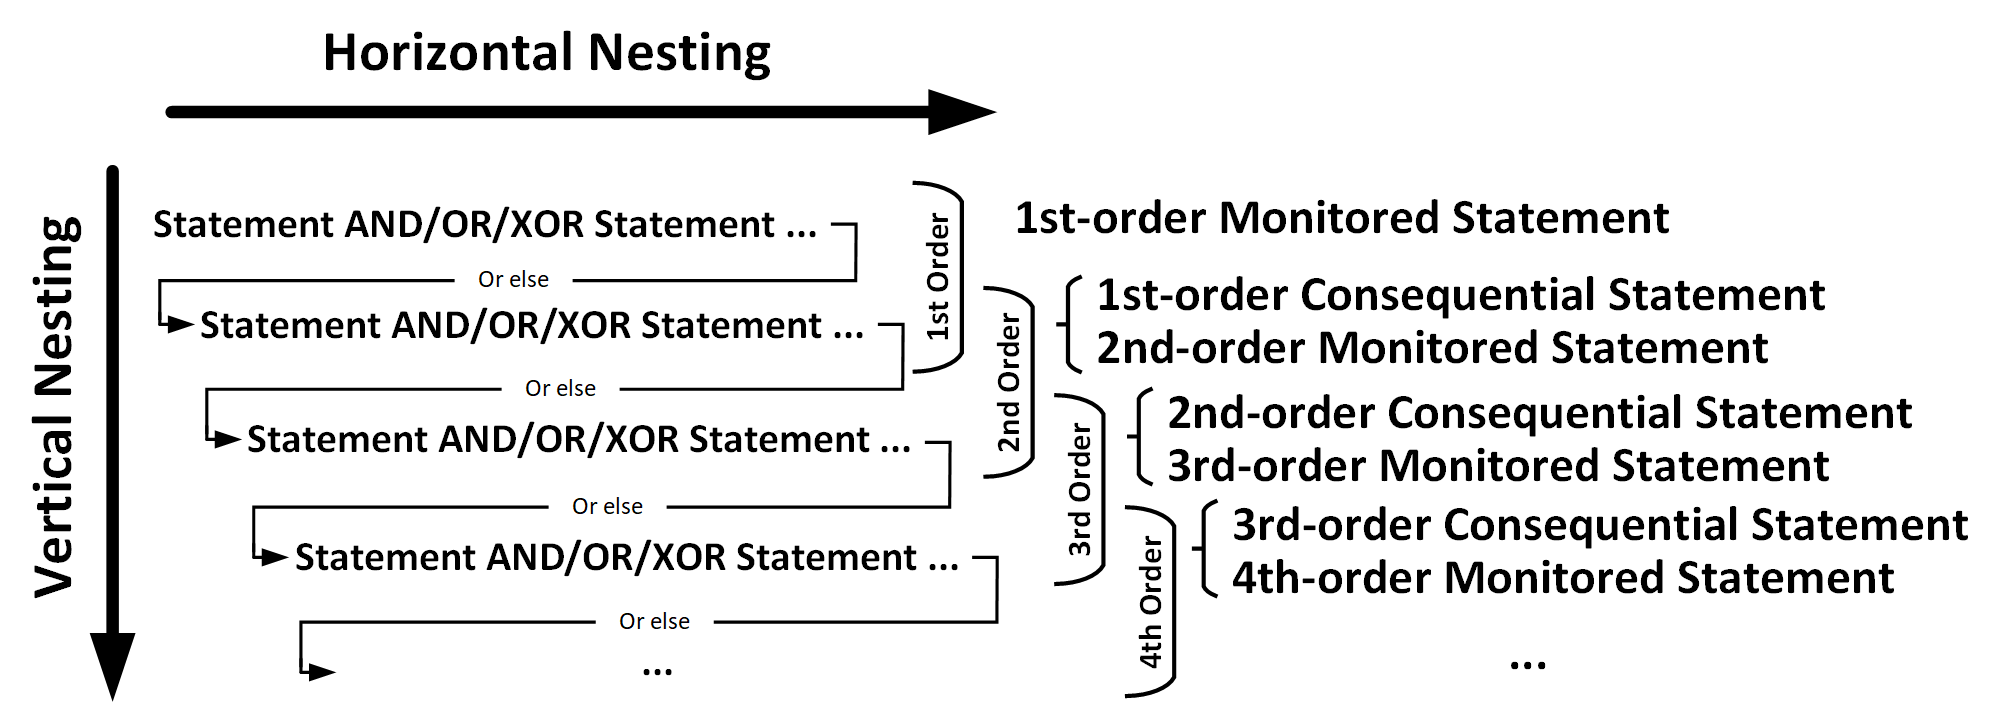
\includegraphics[width=0.8\textwidth]{figures/NestingPrinciples.png}}
    \caption{Institutional Grammar Nesting Principles}
    \label{fig:NestingPrinciples}
\end{figure}

\subsubsection{Component-Level Nesting}
\label{subsec:ComponentLevelNesting}

In addition to the nesting of statements, IG 2.0 further recognizes the possibility of nesting on individual components. Specific components may be substituted with entire institutional statements, or generalizable instances of activity (e.g., statements of fact, observed behavior) expressed in the syntactic form of institutional statements. For regulative statements, those may characterize individuals with respect to their actor properties, embed statements as abstract objects (e.g., the belief that citizens must comply with the law), or express preconditions, i.e., statements whose fulfillment is a precondition for the application of a given statement (as exemplified below).

To motivate this approach explicitly, we will use the following example: \begin{exi}``Organic farmers may sell their produce under the organic label \lb under the condition that organic farmers apply for certification\rb''\end{exi}, with the precondition (the \begin{emp}Activation Condition\end{emp} as a more specific variant of the Context component, as to be discussed in \cref{subsec:ActionSituation}) identified in braces. Rewriting this statement for illustration, we find the following component characterization: 

\begin{itemize}
\itemsep0em
\item Attributes: Organic farmers
\item Deontic: may
\item Aim: sell
\item Direct Object: their produce
\item Execution Constraint (Context): under the organic farming label
\item Activation Condition (Context):\footnote{The activation condition and execution constraint components are a specialization of the Context component, which will be introduced at greater detail in \cref{subsec:ActionSituation}.} under the condition that organic farmers apply for certification
\end{itemize}

Here the instance of behavior embedded in the activation condition reflects the precondition, but, upon closer inspection, may in itself be expressed in terms of syntactic components of institutional statements, either reflecting a specific action configuration (as statement of fact, behavioral instance, or observation) or an institutional statement in its own right (including combinations of statements). 

We refer to cases where individual components of an institutional statement can be replaced by institutional statements (or statements that follow the syntactic structure of institutional statements) as \begin{emp}component-level nesting\end{emp}\index{Component-Level Nesting}. An institutional statement that contains any such nested structure (as initially indicated in \cref{subsubsec:AtomicInstitutionalStatements}) is not atomic in kind. 

Expanding the statement above correspondingly, we arrive at the following structure exemplifying the nesting on the activation condition:

\begin{itemize}
\itemsep0em
\item Attributes: Organic farmers
\item Deontic: may
\item Aim: sell
\item Direct Object: their produce
\item Execution Constraint (Context): under the organic farming label
\item Activation Condition (Context): under the condition that 
\begin{itemize}
\item Attributes: organic farmers 
\item Aim: apply
\item Direct Object: for certification
\end{itemize}
\end{itemize}

The use case for such component-level nesting further includes the articulation of abstract concepts, including non-physical concepts (e.g., beliefs, suspicions, etc.) about individuals' behaviors inasfar as those are relevant to capture the institutional setting accurately (e.g., an official may sanction an individual if the official believes that the individual has performed a violation).

Exemplifying nesting on the object component, we can use the statement \begin{emp}``Inspectors must ensure that organic farmers comply with organic farming regulations''\end{emp}. In this instance, the nesting occurs on the object component, i.e., the receiver of the action \begin{emp}ensure\end{emp}, as visualized below.

\begin{itemize}
\itemsep0em
\item Attributes: Inspector
\item Deontic: must
\item Aim: ensure
\item Direct Object: 
\begin{itemize}
\itemsep0em
\item Attributes: organic farmers 
\item Aim: comply
\item Direct Object: organic farming regulations
\end{itemize}
\item (Implied) Context: under all conditions
\end{itemize}

While not motivated further at this stage, component-level nesting (as statement-level nesting) equally applies to regulative and constitutive statements. Component-level nesting can apply to Attributes, Objects, Context components (Activation conditions and Execution constraints) in regulative statements, as well as to Constituted Entity, Constituting Properties and Context components in constitutive statements. It can further be applied in combination with all forms of statement-level nesting, including the further nesting within component-level nested statements. (For example, imagine a chain of preconditions expressed in nested statements). 

The coding for all forms of nesting and combinations thereof, as conceptually described here, is specified in \cref{sec:CodingGuidelines}.

\subsection{Object-Property Hierarchy}
\label{subsec:AttributeObjectHierarchy}

In addition to the nesting concepts, advanced coding relies on decomposing actors and objects into core descriptors and associated properties. For this purpose, we rely on the conceptual representation of an \begin{emp}Object-Property Hierarchy\end{emp}\index{Object-Property Hierarchy} as exemplified in \cref{fig:ObjectPropertyHierarchyExample}. In this visualization, statements such as \begin{exi}``\dots~a written notification of proposed suspension or revocation of certification \dots''\end{exi} reflect an involved Object hierarchy centering on the \begin{exi}``notification''\end{exi}, that has a property \begin{exi}``written''\end{exi}. Looking at the context of the notification we recognize the concept of \begin{exi}``certification''\end{exi} that has the property of being \begin{exi}``suspended''\end{exi} or \begin{exi}``revoked''\end{exi}, expressed as dependent Objects (\begin{exi}``suspension''\end{exi}, \begin{exi}``revocation''\end{exi}), whereas the latter concepts themselves have a shared property of being \begin{exi}``proposed''\end{exi} in the first place. However, while the property \begin{exi}``written''\end{exi} functionally depends on the \begin{exi}``notification''\end{exi}, that is, writtenness alone does not make sense with an Object it refers to, the existence of a certification does not rely on the notification (i.e., it is functionally independent), and has a self-contained property hierarchy (suspended, revoked, proposed) as described above. 

Interpreting complex Object specifications with this decomposition hierarchy in mind affords a uniform coding approach. The structure of this hierarchy for the specific statement is shown in \cref{fig:ObjectPropertyHierarchyExample} (the dashed line signals relationships between functionally independent Objects). Note specifically the potential use of logical operators (\begin{exi}``XOR''\end{exi}), as well as the ability to reflect shared properties (\begin{exi}``proposed''\end{exi}), to disambiguate the logical relationship between the identified properties, an aspect that is implicit in the textual representation. 

\begin{figure}[h!]
    \centering
    \framedfigure{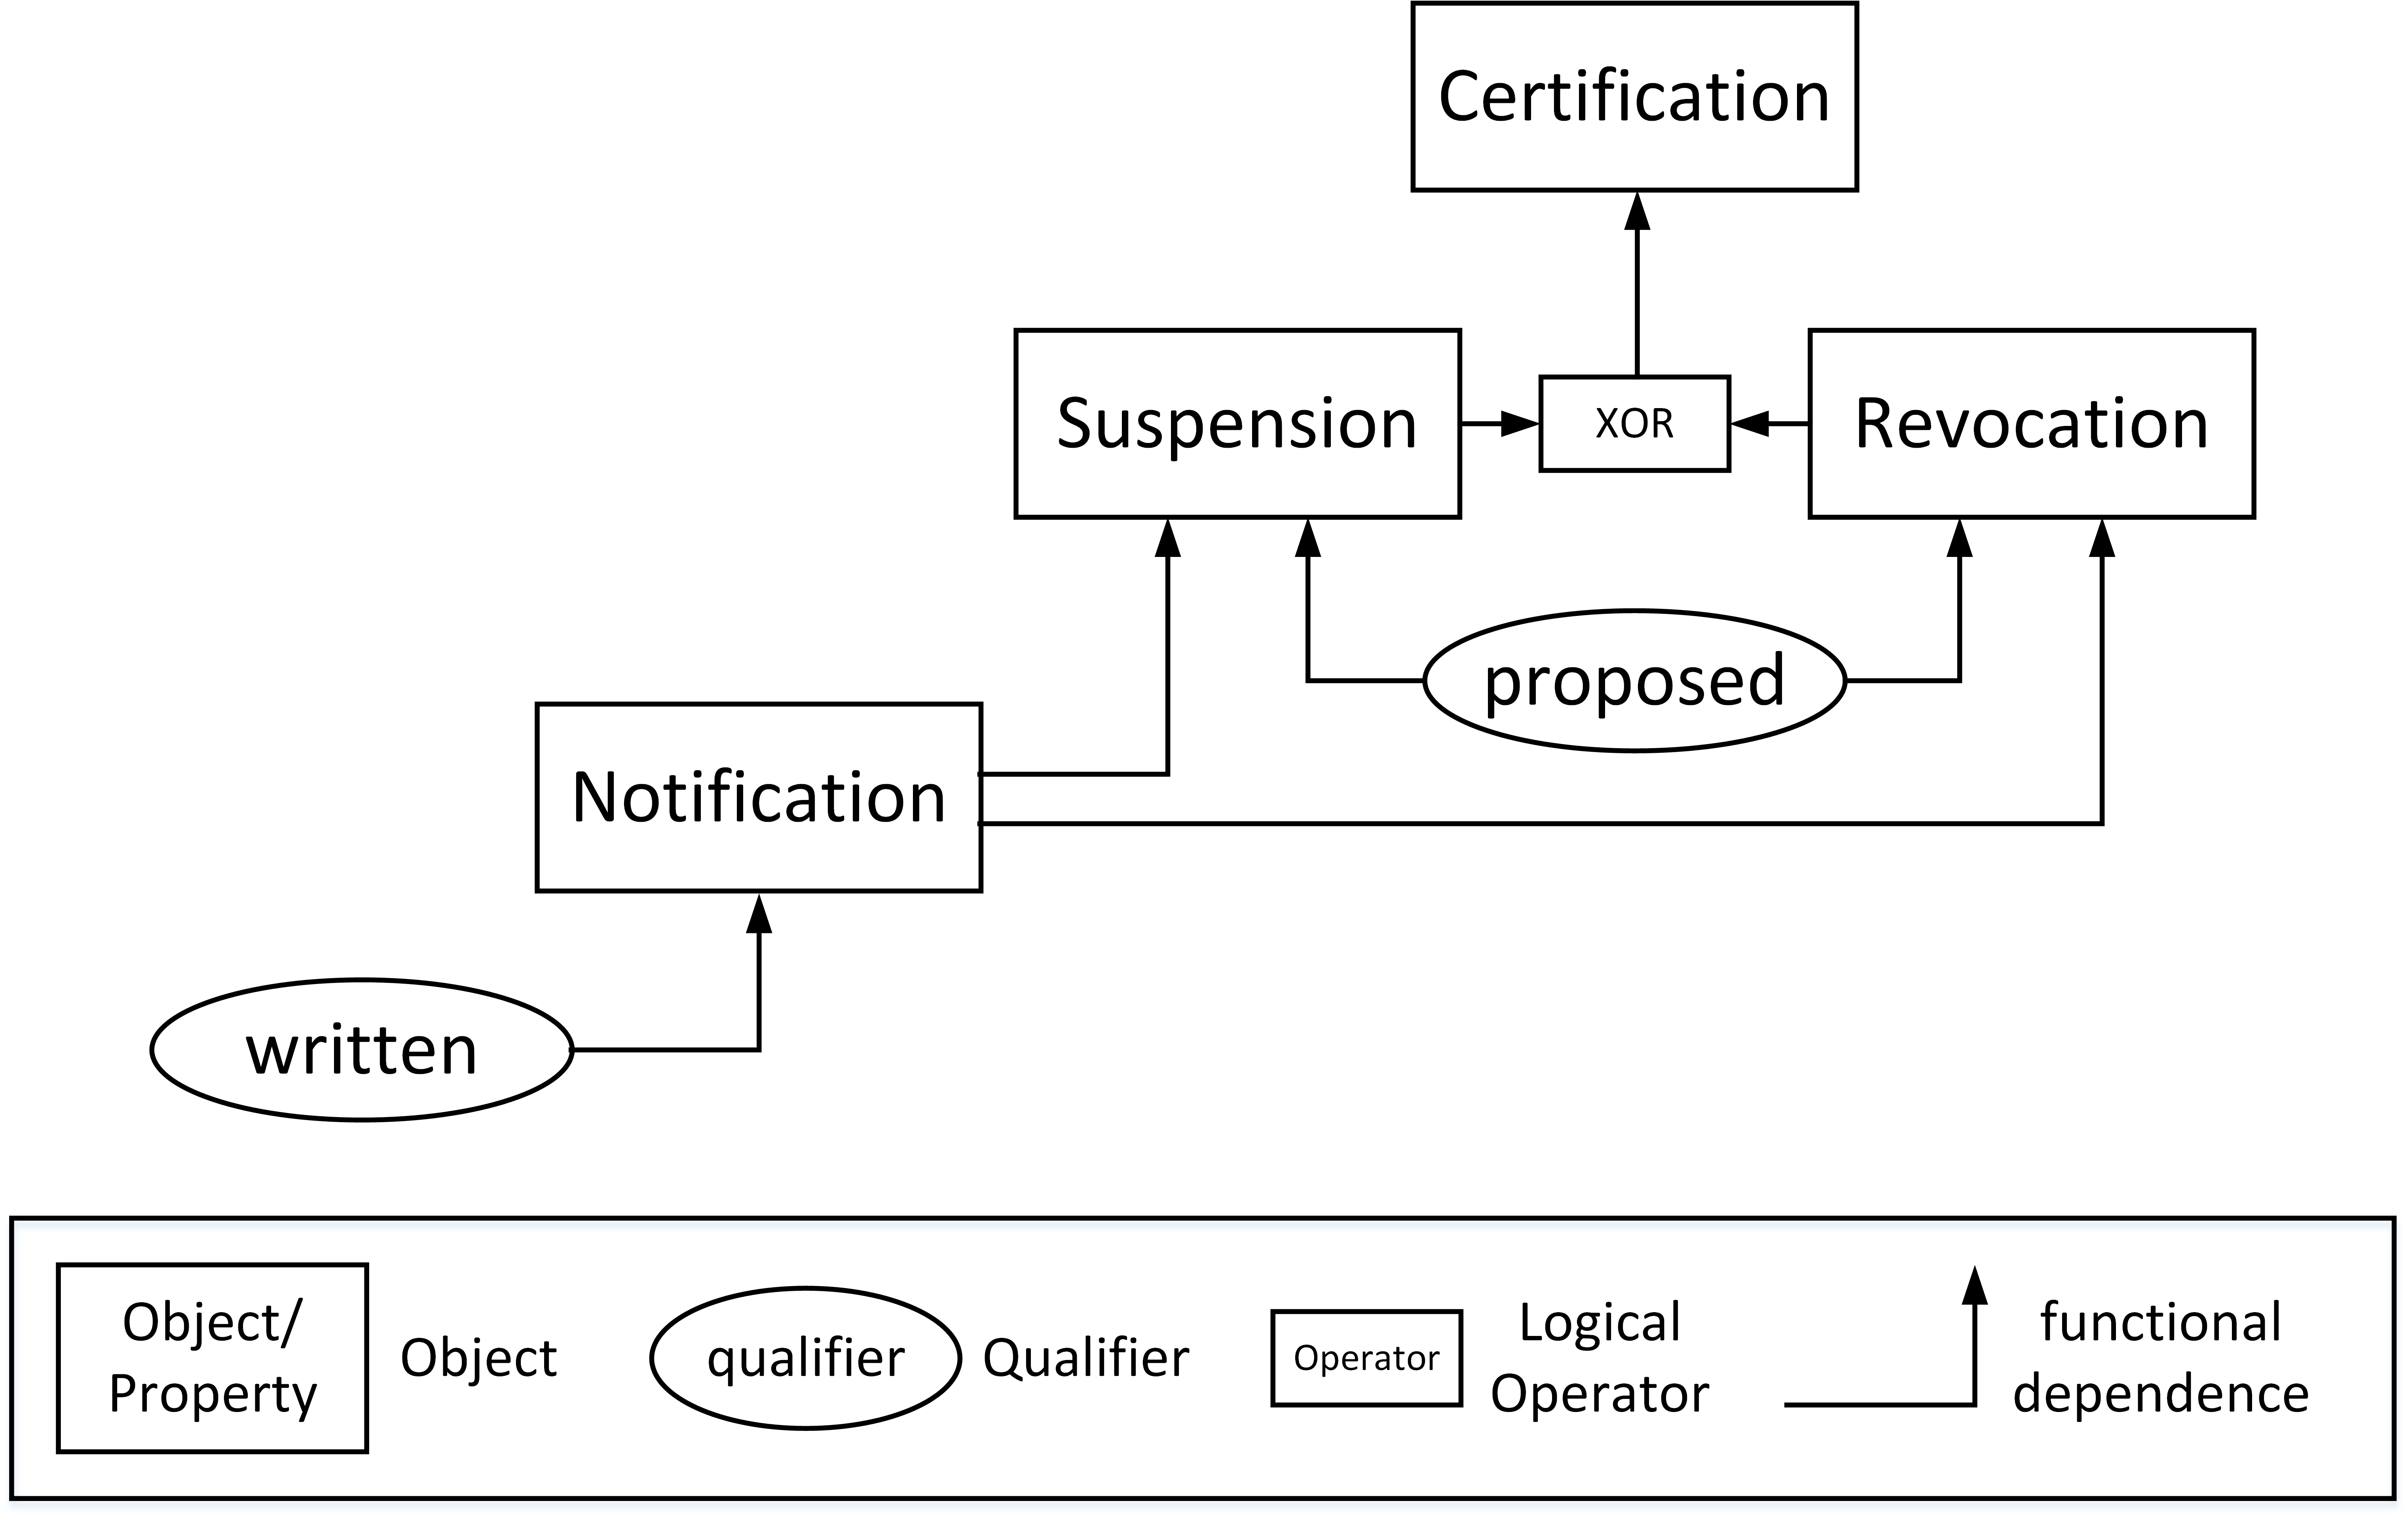
\includegraphics[width=0.65\textwidth]{figures/ObjectPropertyHierarchyExample.png}}
    \caption{Object-Property Hierarchy for the given Example}
    \label{fig:ObjectPropertyHierarchyExample}
\end{figure}

Capturing all potential decomposition approaches, we can apply this scheme to functionally dependent properties (\begin{exi}``written''\end{exi} in the previous example), functionally independent Objects or properties (\begin{exi}``certification''\end{exi} in the previous example), and furthermore afford the substitution of Objects by complete institutional statements. Since the latter aspect relies on richer contextualization, it will be exemplified in the context of the coding instructions. The stylized general form of the \begin{emp}Object-Property Hierarchy\end{emp} is shown in \cref{fig:ObjectPropertyHierarchy}. Note that logical operators apply to both functionally dependent and independent properties and on any level of decomposition.

\begin{figure}[h!]
    \centering
    \framedfigure{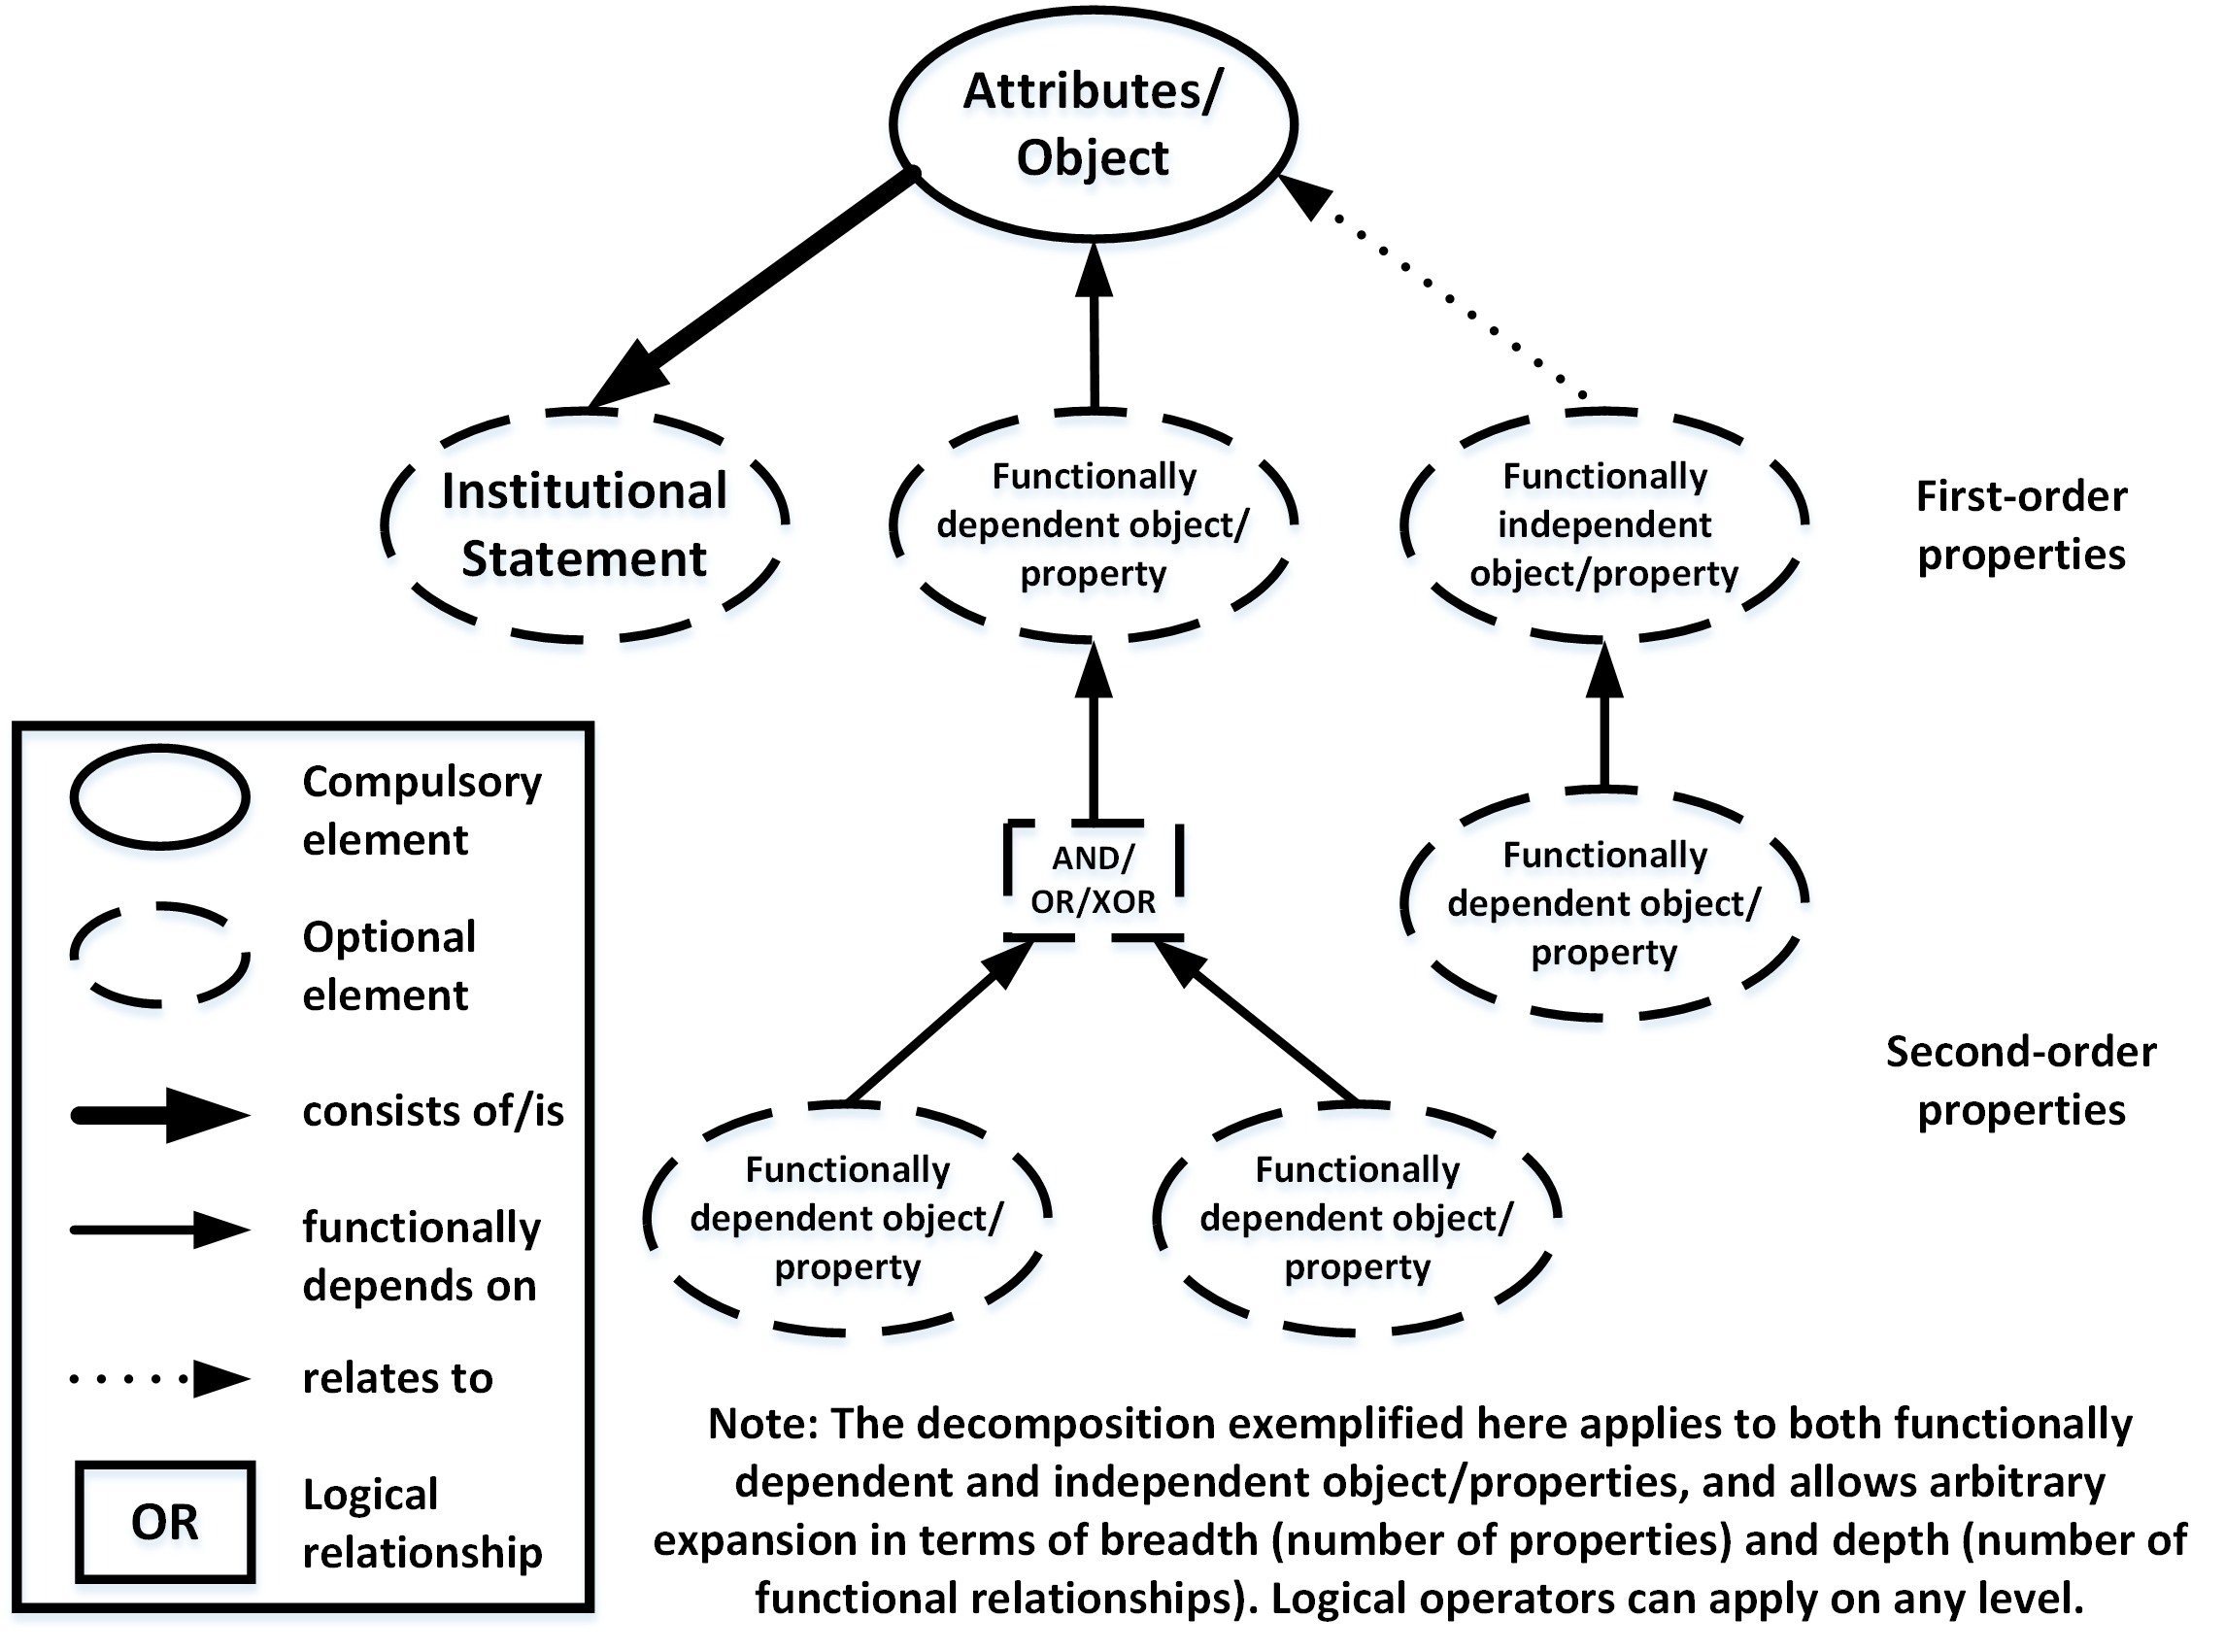
\includegraphics[width=0.55\textwidth]{figures/ObjectPropertyHierarchy.png}}
    \caption{Object-Property Hierarchy}
    \label{fig:ObjectPropertyHierarchy}
\end{figure}

\newpage

\subsection{Relating Institutional Statements to Action Situations}
\label{subsec:ActionSituation}

A concept central to the coding with IG 2.0 is the action situation~\citep{Crawford2005}. Basically, an action situation is defined as an institutionally governed setting in which two or more actors interact, in relation to which specific outcomes emerge. Action situations are governed by a configuration of different types of institutional statements, which can be regulative or constitutive in kind, with distinctive functional properties. The seven types of institutional statements\index{Rule types}, labeled in parentheses in terms of different types of ``rules'', convey: positions that actors can occupy within an action situation (position rules), eligibility criteria for occupying those positions (boundary rules), operational actions linked to actors occupying certain positions (choice rules), situational outcomes (scope rules), channels of information flow (information rules), guidance on collective decision making (aggregation rules), and incentives tied to particular actions (pay-off rules). Each action situation can be governed by multiple statements of a particular type.  Action situations, and key action situation components, are schematically visualized in \cref{fig:ActionSituation}. In the widest sense, action situations describe the context in which institutional statements operate, and in the context of regulative statements, specifically the mapping between actors, actions, outcomes and the associated payoffs.

\begin{figure}[h!]
    \centering
    \framedfigure{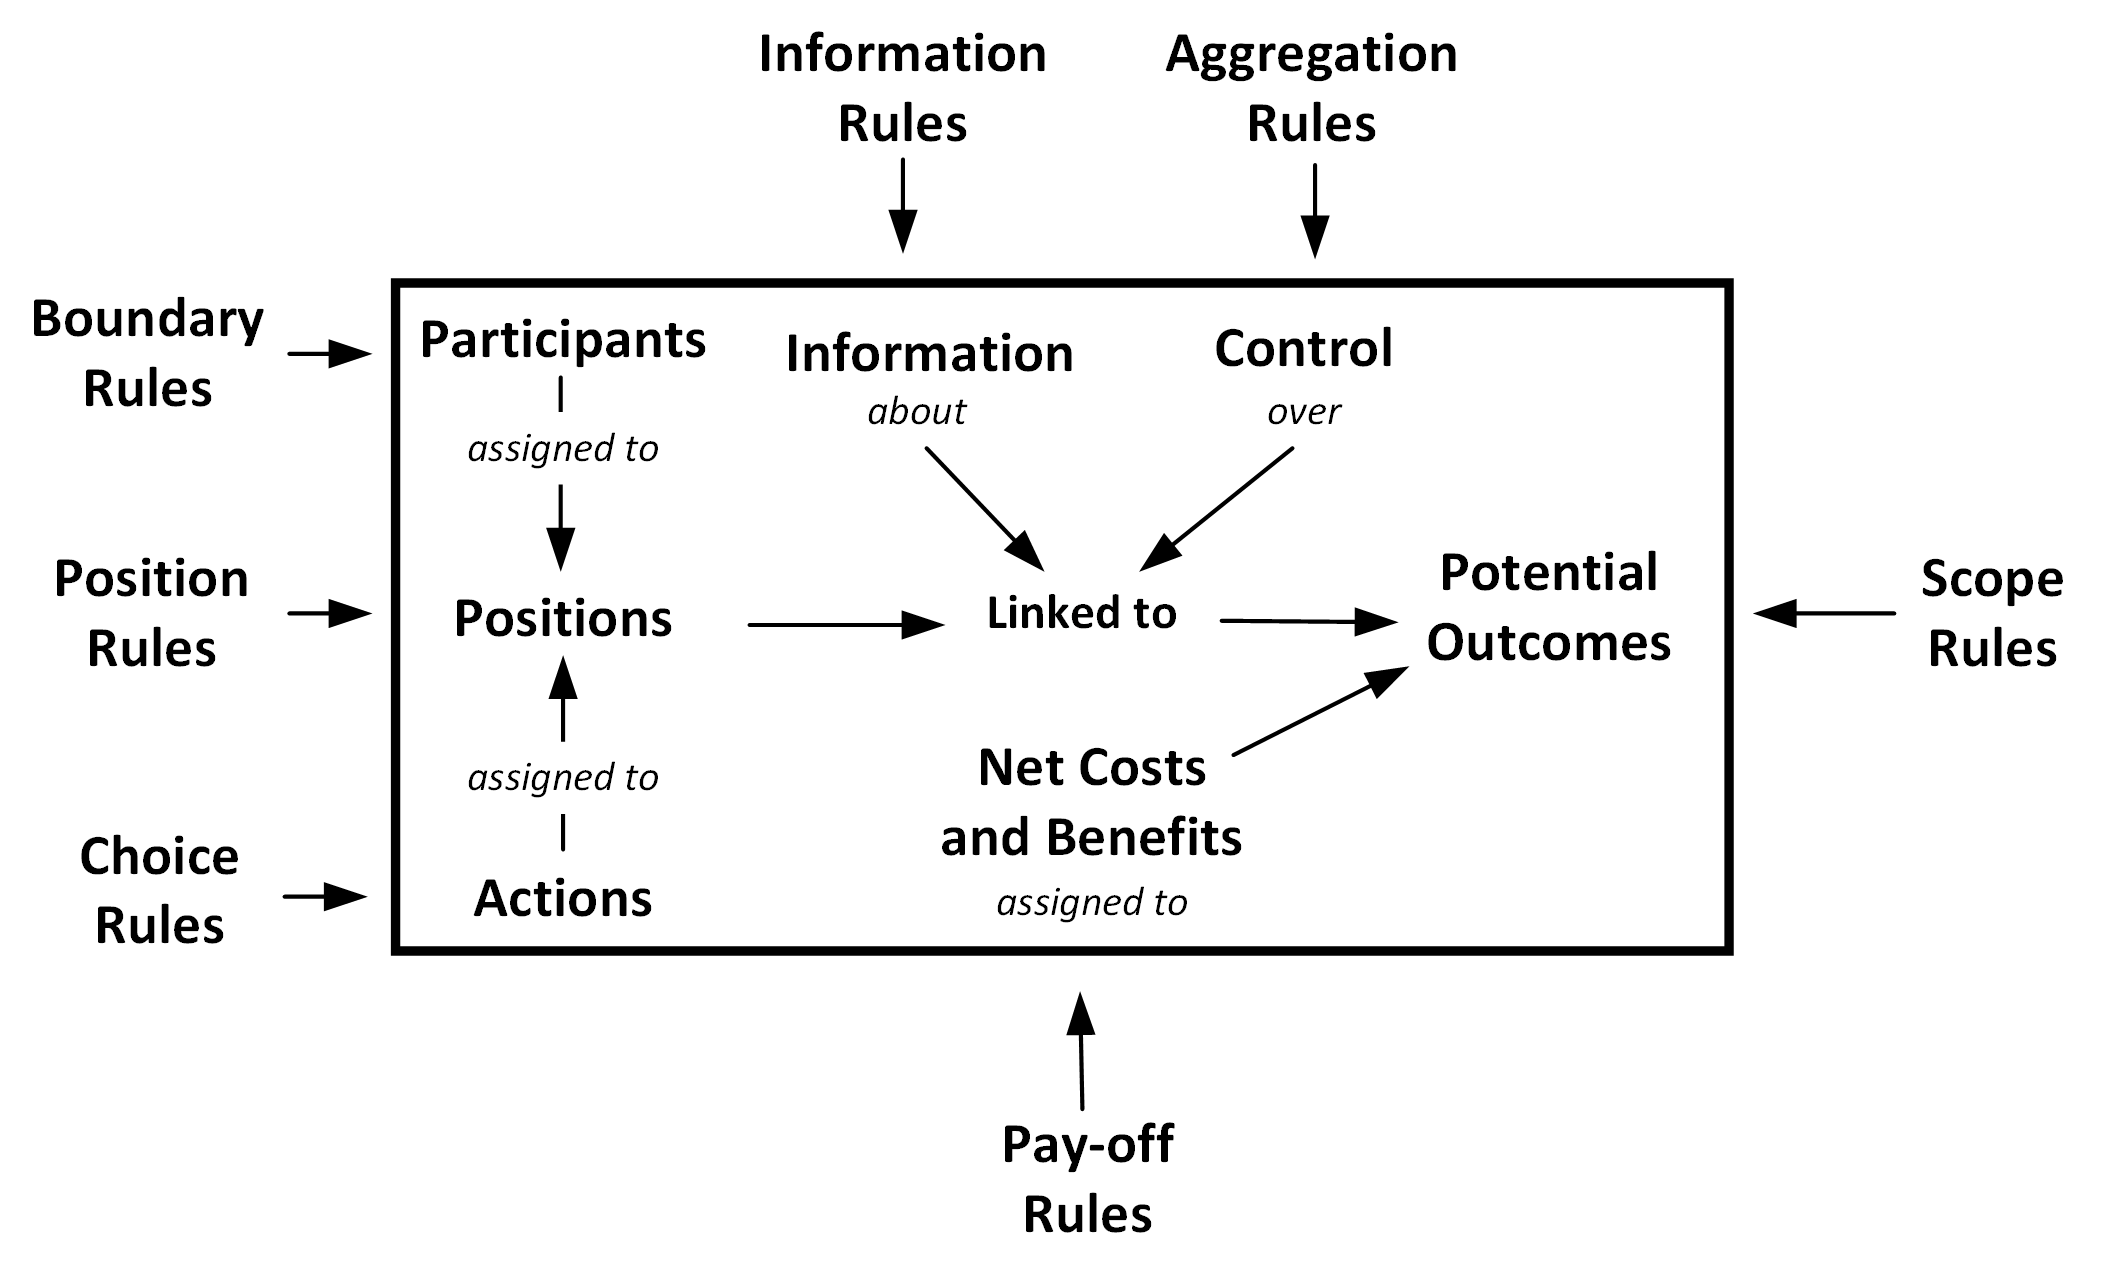
\includegraphics[width=0.8\textwidth]{figures/ActionSituation.png}}
    \caption{Schematic Visualization of the Action Situation (as per \citet{Crawford2005})}
    \label{fig:ActionSituation}
\end{figure}

Again, the rule type taxonomy associated with the action situation concept links to the IG insofar as whole institutional statements can be classified accordingly, depending on their functional properties. 

The IG 2.0 specification leverages the action situation concept in recognizing generally that institutional statements characterize activity occurring in action situations, and in accounting through syntactic classification for ways that institutional statement information corresponding to the Context component contextualizes intra- and inter-statement activities. 

Operationalized in the context of regulative statements, Context clauses can instantiate an action situation in which an Attribute acts on Objects in a particular manner, and which are governed by some configuration of institutional statements. By way of contrast, the Context clauses of other statements may simply constrain an Attribute’s behavior in some way within a given action situation. As noted in \cref{subsec:Syntax}, context clauses which serve an instantiation function, as well as Attribute or Object changes are referred to as Activation Conditions\index{Activation conditions}. Context clauses which qualify action are referred to as Execution Constraints\index{Execution constraints}. \cref{fig:ActionSituationConditionsConstraints} schematically represents how Activation Conditions and Execution Constraints situate relative to action situations. 

\begin{figure}[h!]
    \centering
    \framedfigure{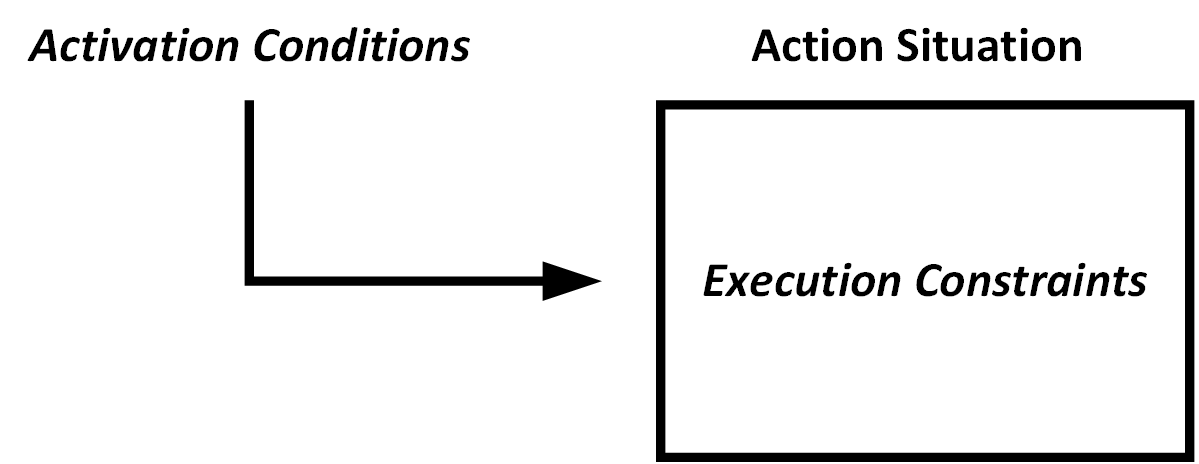
\includegraphics[width=0.5\textwidth]{figures/ActionSituationConditionsConstraints.png}}
    \caption{Activation Conditions and Execution Constraints Principles}
    \label{fig:ActionSituationConditionsConstraints}
\end{figure}

Naturally, explicit characterization of how institutional statements relate to action situations necessitates understanding of the institutional domain. Without this, the coder may encounter difficulty in determining as to whether a specific Context descriptor refers to the action situation more generally, or the action specifically in the form of an action property. While we offer further elaboration as part of the coding guidelines in \cref{sec:CodingGuidelines}, we provide a brief example to motivate the distinction at this stage. 

Inherent to the Activation Condition is reference to a set of exogenous variables; exogenous in the sense that it references states or actions that are beyond the actions that can be qualified within certain Execution Constraints in an instantiated environment (e.g., a new action situation, an environment in which Attributes change or take on new roles, or an environment in which Attributes act in an altered way upon Objects). In other words, Activation Conditions precede the regulated action and activate a given institutional statement in the first place. Conversely, Execution Constraints describe constraints on actions once enacted (and implicitly on actors and associated pre-/proscription as visualized in \cref{fig:ActionSituationContextRelationships}). 

\begin{figure}[h!]
    \centering
    \framedfigure{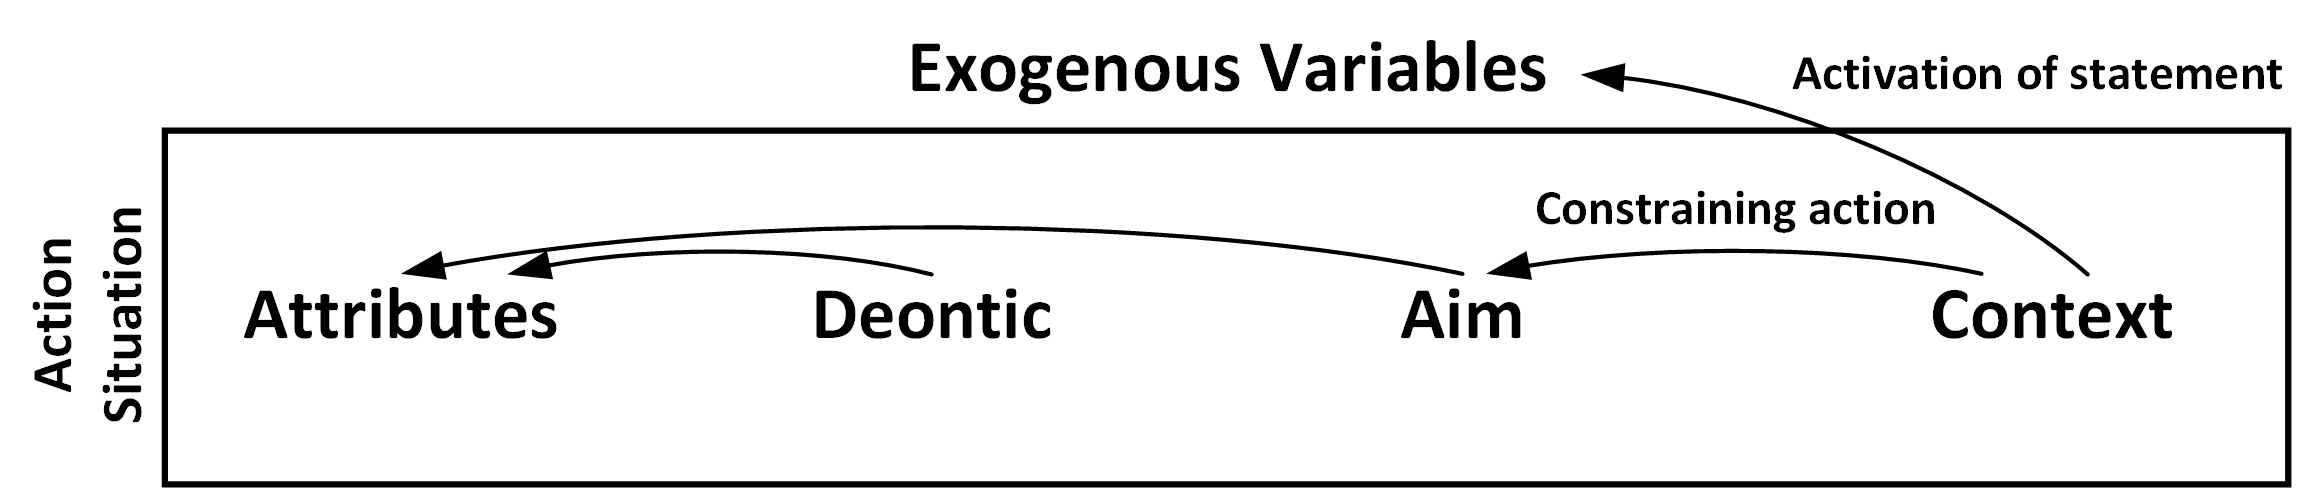
\includegraphics[width=0.9\textwidth]{figures/ActionSituationContextRelationships.png}}
    \caption{Context Relationships in the Action Situation}
    \label{fig:ActionSituationContextRelationships}
\end{figure}

Procedurally, this implies different semantics for Activation Conditions and Execution Constraints. Activation Conditions represent Context external to the action situation an institutional statement is embedded in that activates the non-conditional part of an institutional statement, and possibly leading to the activation or modification of an action situation. Execution Constraints, in contrast, are directly attached to the institutional statement and thus reflect context embedded within the action situation itself. The discussed distinction is summarized in \cref{fig:ActionSituationContextRelationships}. 

Offered here is more operational guidance on the differentiation highlighted above, which starts with  the identification of Context clauses in an institutional statement. To systematize the differentiation, we firstly provide a terminological basis. Linguistically, context clauses are generally modifiers, specifically qualifiers (\begin{emp}``usually''\end{emp}, \begin{emp}``some''\end{emp}, \begin{emp}``annually''\end{emp}), adverbial clauses (\begin{emp}``When the traffic light turns from red to green, \dots''\end{emp}) and prepositional clauses (\begin{emp}``after midnight''\end{emp}). Whereas qualifiers reliably signal Execution Constraints (action properties in the narrow sense), and adverbial clauses generally indicate Activation Conditions, depending on contextual interpretation, prepositional clauses can fall in either category and selectively signal Activation Conditions or reflect Execution Constraints (action properties in the wider sense). 

The differentiated treatment for prepositional clauses is best described with an example: \begin{emp}``At 8am, farmers may begin selling their goods in accordance with market rules,''\end{emp} contains two context clauses (\begin{emp}at 8am, in accordance with market rules\end{emp}), one of which is a conditions clause (\begin{emp}at 8am\end{emp}) and one of which is a constraints clause (\begin{emp}in accordance with market rules\end{emp}). Context clauses may be implicit, and institutional statements are not constrained in the number of clauses for condition and constraint type. The remainder of the statement is the non-context clause of an institutional statement. \cref{fig:ContextClausesInInstitutionalStatement} highlights this decomposition of regulative institutional statements with respect to the Context component.

\begin{figure}[h!]
    \centering
    \framedfigure{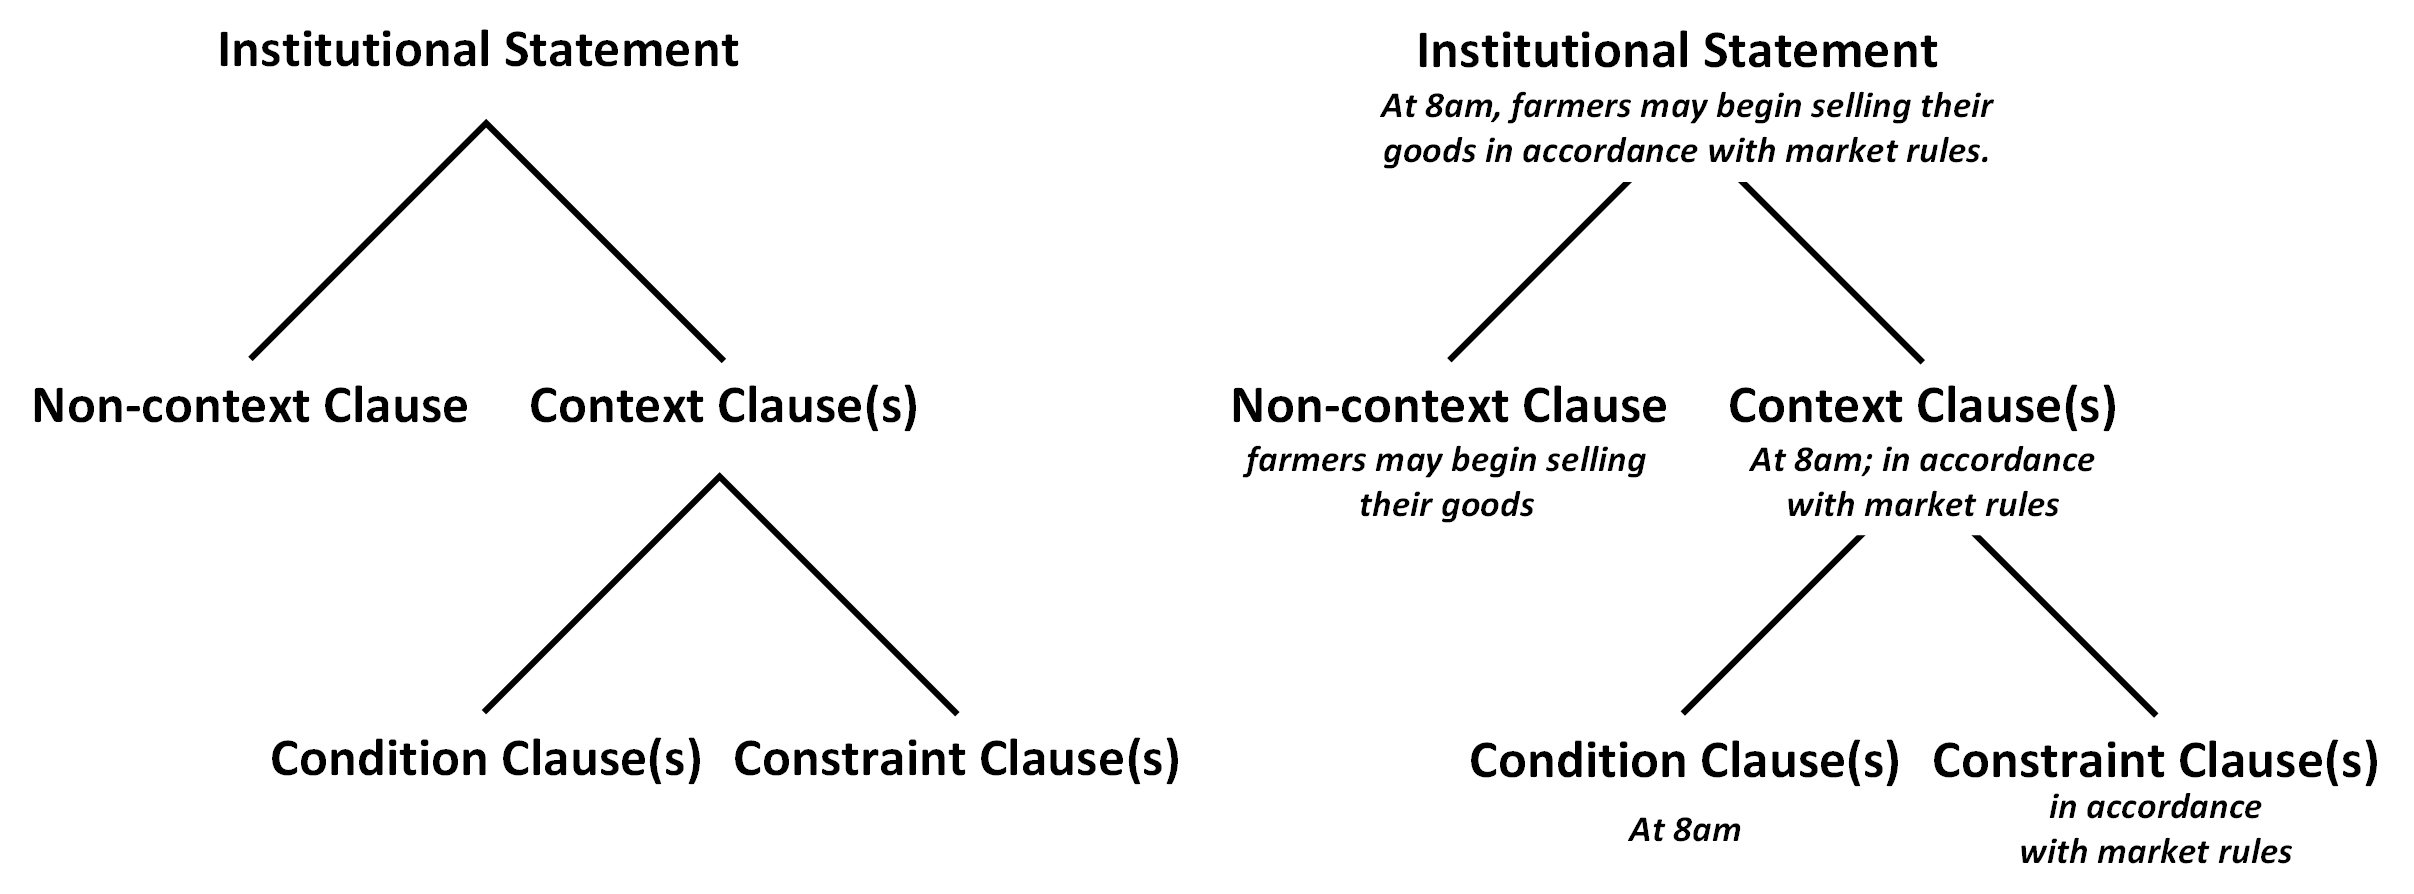
\includegraphics[width=0.95\textwidth]{figures/ContextClauses.png}}
    \caption{Context Clauses in Institutional Statements}
    \label{fig:ContextClausesInInstitutionalStatement}
\end{figure}

Decision heuristics can be employed to aid in the identification of activation conditions and execution constraints. The following heuristics are particularly designed to help the analyst determine if a context clause in question is an activation condition, leaving the resultant classification of the clause as an execution constraint, if it is determined that it is not. Offered first is a heuristic that generalizes across regulative and constitutive statements. This is followed by heuristics specific to two different types of statements. 

\begin{ptit}General Heuristic for Identifying Activation Conditions:\end{ptit} 

The clause instantiates a discrete setting (constrained temporally, spatially, or otherwise as shown below) and/or event that activates the non-condition clauses of the institutional statement (i.e., non-context clauses along with potential constraint clauses) as a whole.
The following example statements contain activation conditions (underlined) for illustration.:
\begin{itemize}
    \item \begin{emp}``Upon receiving final notice of non-compliance, farmers shall cease sale of any product bearing the USDA organic farming label.''\end{emp} This statement signals the instantiation of a novel attribute-object link described by the activity, and is positioned within a discrete temporal setting.
    \item \begin{emp}``Starting January 1, the Department of Agriculture is the certifying authority.''\end{emp} Here the statement makes explicit reference to an event that leads to the activation of an associated role change in a constitutive statement.
    \item \begin{emp}``Upon entry into the house, visitors must remove shoes.''\end{emp} (Event) vs. \begin{emp}``At home individuals must not wear shoes.''\end{emp} (Discretized setting). Whereas the first statement references a specific event (entry), the second statement describes a general discretized setting in which the statement holds at all times, i.e., the statement is activated at any time.
\end{itemize}

\begin{ptit}Heuristics for Identifying Activation Conditions in Regulative Statements:\end{ptit}

\begin{emp}Attributes\end{emp}: The clause instantiates a) a change in attributes linked to a statement's activity or b) a change in attribute role.
\begin{itemize}
    \item \begin{emp}``Between the hours of 6pm and 6am on Mondays, members of neighborhood watch residing in blocks 7-10 will assume night patrol activities.''\end{emp} This example signals a change in attribute role within a specified time frame.
\end{itemize}

\begin{emp}Objects\end{emp}: The clause instantiates a change of the object(s) linked to the statement's activity.
\begin{itemize}
    \item \begin{emp}``Starting Dec.~15th, inspectors must exclusively use the revised inspection form.''\end{emp} (novel object use)
\end{itemize}

To support the classification more generally, we can further offer practical considerations to aid in the decision making: 

\begin{itemize}
    \item Regulative statements: More generally, in a regulative context with a given specification of pre/proscriptions, activation conditions constitute a discretized setting in which institutional content can in principle be adhered to or violated.
    \item Context-clause interdependencies: If the  application of the clause of concern is contingent on the prior activation of another context clause, the former is an execution constraint, whereas the latter describes an activation condition in the context of the analyzed institutional statement. If only the satisfaction of both clauses leads to the activation of the non-context clause, both are sensibly identified as activation conditions.
    \begin{itemize}
        \item Example: \begin{emp}``When live fish or viable gametes are sold, traded, taken or otherwise disposed of from an aquaculture facility, the permittee or operator shall, at the time of transfer of possession, give an invoice to the person receiving such fish or viable gametes.''\end{emp} Here \begin{emp}``when live fish \dots facility''\end{emp} represents the activation condition; the subsequent provision of an invoice \begin{emp}``at the time of transfer of possession''\end{emp} is an execution constraint.
    \end{itemize}
\end{itemize}

Returning to the initial example \begin{emp}``At 8am, farmers may begin selling their goods in the farmer's market.''\end{emp}, the condition clause \begin{emp}``At 8am''\end{emp} signals the instantiation of a discrete temporal setting in which the remaining statement is activated as a whole (i.e., permitting the sales of goods on the market). The clause \begin{emp}``in the farmer's market''\end{emp} complements the description of the regulated content and neither affects attribute/role, object nor does it define a setting that activates the remaining statement. The resulting statement would thus be coded as follows:

\begin{exa}
Coded statement: ``At 8am (Activation statement), farmers (Attribute) may (Deontic) begin selling (Aim) their goods (Object) at the farmer’s market (Execution constraint).''
\end{exa}

To highlight the distinction between activation conditions and execution constraints more clearly, we can review the following statement: \begin{emp}``Farmers may sell non-organic goods in the organic farmer's market only between the hours of 3 and 5pm.''\end{emp}

Here the time frame \begin{emp}``between the hours of 3 and 5pm''\end{emp} signals a distinctively different relationship between attributes (farmers), aim and object, whereas the \begin{emp}``in the farmer's market''\end{emp} complements the characterization of the institutional setting in which the permission holds. 

This is in contrast to the following statement:
\begin{exa}``\underline{Farmers must perform inventory of goods sold} at farmers market daily.'' (execution constraint)\end{exa} 
This statement signals a general obligation to provide inventory information (i.e., is activated at all times), but does not establish a specific discretized setting or event that triggers the obligation.

Contrasting this, the following example highlights such event, leading to the characterization of the conditional clause as activation condition:
\begin{exa}``At the close of market each day (activation condition), \underline{farmers must perform inventory of goods sold}.''\end{exa}

\begin{ptit}Heuristics for Identifying Activation Conditions in Constitutive Statements:\end{ptit}

\begin{itemize}
    \item \begin{emp}Entity\end{emp}: The clause instantiates a change in the Entity that is being constituted. 
    \begin{itemize}
        \item Example: \begin{exa}``In the event that the Board Chair position becomes vacant, the Vice-Chair is the chief executive of the Council.''\end{exa} (change in entity specification under event)
    \end{itemize}
    \begin{emp}Properties\end{emp}: The clause instantiates a change in the constituting properties of the entity that is constituted, reconstituted or otherwise affected in the institutional statement.
    \begin{itemize}
        \item Example: \begin{exa}``Starting Dec.~15th, organic farming is agricultural production that does not involve the use of synthetic chemicals or genetically modified organisms.''\end{exa} (change in constituting properties of constituted entity)
    \end{itemize}
\end{itemize}

\begin{ptit}Considerations for challenges cases:\end{ptit}

In written institutional statements, it is not uncommon to find constructions that elevate a statement's pre- or proscriptiveness embedded in activation condition or execution constraint. A stylized example is the following statement: \begin{exa}``Drivers must comply with traffic rules, especially when encountering congested traffic.''\end{exa}

A specific characteristic of such statement is the elevated prescriptiveness based on the context clause, with specific focus on the contextual characterization \begin{exi}``\dots~especially when encountering congested traffic''\end{exi}. As such, the context characterization signals a situational increase of prescriptiveness, beyond the generally expected compliance. Facing such statements, the analyst will need to evaluate, whether this statement exclusively highlights such contextual elevation, which is interpreted as an execution constraint, or characterizes a specific condition under which the non-context part of a statement applies as a whole. Typical terms associated with elevated prescriptiveness mediated via execution constraints include 

\begin{itemize}
    \item especially
    \item particularly
    \item specifically
\end{itemize}

Activation conditions are conventionally signaled using terms such as

\begin{itemize}
    \item where possible
    \item under the condition
    \item when \dots
\end{itemize}



\newpage

\subsection{Institutional Statement Type Heuristics}
\label{subsec:StatementTypesHeuristics}

IG 2.0 has been developed in response to observed challenges in the encoding of policy, such as the inability to sensibly capture institutional statements of constitutive kind. In addition to affording the syntactic parsing of constitutive institutional statements, their unambiguous characterization is of central importance so as to ensure coding reliability.

While a characterization based on syntactic alignment has an intuitive appeal, not in all instances does this lead to correct statement classification, e.g., based on contextually implied actor associations or stylistic artifacts. To afford a reliable characterization of statements, we rely on a set of first principles expressed in a set of general guidelines that seek to identify both constitutive and regulative statements, alongside potential combinations of those, the expression of which IG 2.0 explicitly supports. This is then followed by a more specific set of questions, supporting the identification of individual features relevant for a distinctive statement characterization.

To lend best possible guidance, the guidelines, or heuristics, are expressed as closed questions, alongside clarifying explanations.

\begin{ptit}General Heuristics for Identifying Institutional Statement Types:\end{ptit}

\begin{itemize}
\item Does the statement introduce or parameterize fundamental aspects of the action situation (boundaries, definition or modification of actors, actions, objects, artifacts and associated affordances; endowment of rights or authority/power), and in doing so, define positioning and constellation of entities in an institutional setting in which potentially regulated behavior is enacted? $\rightarrow$ If so, the statement is \begin{emp}constitutive\end{emp} in kind.
\item Does the statement signal unambiguously implied or explicit agency, while  specifying duty and discretion, or sanctions for transgression? In doing so, does the statement draw on (i.e., makes implicit or explicit reference to) actors, objects or artifacts, including a potential modification of the institutional setting as an outcome of actors exercising activities regulated as part of the institutional statement? $\rightarrow$ If so, the statement is \begin{emp}regulative\end{emp} in kind.
\item If both criteria are satisfied (e.g., introduction of novel entity as byproduct of enacted agency), test for combination of regulative and constitutive statements under \begin{emp}consideration of the primary and secondary objective/purpose of the statement in the institutional setting as commonly signaled by aim or constitutive function respectively\end{emp} (e.g., essential focus on regulation of behavior vs.~parameterization of institutional setting/action situation -- with further operational criteria provided in \cref{tab:SemanticStatementTypeHeuristics}). 

Statements are then characterized as regulative-constitutive (where regulation is of primary concern), or constitutive-regulative hybrid (where parameterization is of primary concern), respectively (see \cref{subsec:ConstitutiveRegulativeHybrids} for more details on hybrid institutional statements).

A special case are statements that can coded according to both syntactic forms. Where dual coding of statements is possible and desirable (i.e., coding as \begin{emp}both\end{emp} constitutive and regulative statements), statements can be encoded as polymorphic institutional statements (see \cref{subsec:SyntacticPolymorphs}). 

Where a specific preference for regulative or constitutive forms exists based on analytical preferences, this poses challenges to coding reliability, an aspect that can be alleviated by defining a specific \begin{emp}interpretational scope\end{emp} prior to coding (as described in the following).

\end{itemize}

\fcolorbox{black}{\boxbgcolor}{\begin{minipage}{16.5cm} %{15.5cm}
\hypertarget{tablink:InterpretationalScopeOfInstitutionalStatements}{\begin{ptit}Interpretational Scope of Institutional Statement Coding\end{ptit}}

To establish a reliable and consistent encoding of institutional statements, an important concern is the appropriate characterization of the intended \begin{emp}scope of interpretation\end{emp} coders should put forth when establishing the structure and type of institutional statements. More specifically, while the encoding of text centers around individual institutional statements as units of analysis, tacit preferences in interpretation can become overt when distinguishing between constitutive and regulative statements. 

Using the following set of (stylized) example statements for illustration, we can observe two leading statements of regulative kind, which, in alignment with the general heuristics expressed above, is signaled by the primary focus on behavior regulation. The last statement, in contrast, offers further contextualization for the previous statements.

\vspace{0.2cm}
%\sp
\begin{exa}
(1) Organic farming operations must not utilize genetically-modified seeds.

(2) Organic farming operations may not process crops other than the ones specified in Appendix A.

\dots

(10) Paragraphs in this section do not apply to traces of genetically modified material.
\end{exa}
%\sp
\vspace{0.2cm}

Exploring the statements structurally, the last statement does not directly regulate behavior, but instead imposes operational constraints on the preceding statements. Given its broader overarching function and associated capacity for re-configuration, it may be interpreted as \begin{emp}parameterizing in nature\end{emp}, since it affects the wider institutional setting regulated in the referenced statements that offer specific operational guidance. Such characterization would lead to a qualification of the statement as \begin{emp}constitutive\end{emp} in kind. 

Conversely, however, the statement can be reconstructed in a form that captures the operational character. Absent specific coding instructions (which are discussed in \cref{sec:CodingGuidelines} onwards), the last statement could be reformulated as

\vspace{0.2cm}
%\sp
\begin{exa}
Organic handling operations may not apply paragraphs in this section to traces of genetically modified material.
\end{exa}
%\sp  % too wide
\vspace{0.2cm}

Following the general heuristics for statement classification, the reformulated statement primarily focuses on behavior regulation, suggesting its characterization as \begin{emp}regulative\end{emp}. 

Without further specification, a potential inconsistent interpretation of statements of such character can lead to reliability challenges, an aspect IG 2.0 seeks to alleviate.

To afford a consistent differentiation that a) establishes reliability, and b) ensures methodological consistency in response to analytical objectives, we differentiate forms of coding by \begin{emp}scope of interpretation\end{emp}, where interpretation of \begin{emp}narrow scope\end{emp} emphasizes an immediate interpretational focus on the statement of concern, including its semantics as well as the function it holds with respect to other statements expressed in the policy, or the policy at large; however, semantic linkages of the statement are not resolved beyond the statement itself. 

Contrasting the narrow scope, applying a \begin{emp}wide scope\end{emp} of interpretation expands the focus of analysis by resolving implied or explicit semantic links to other statements, and thereby introduces potential inferences that can affect the interpretation and representation of the analyzed statement both structurally (as showcased above for the reconstruction in regulative form) and semantically (e.g., by drawing deeper inferences draw from and even extend beyond the linked statement). While rooted in the original institutional statement of concern, coding based on wide scope implicitly invokes the interpretation from a systemic perspective, and thereby introduces a variable unit of analysis; this interpretation is necessarily anchored in, but invariably extends beyond, the originating institutional statement. 

\end{minipage}}

\fcolorbox{black}{\boxbgcolor}{\begin{minipage}{16.5cm}

The choice of interpretational scope is an important consideration and determined as part of the design of the coding exercise, alongside aspects such as pre-coding steps (see \cref{sec:PrecodingSteps}), prior to operational coding. Justifications for either choice of interpretational scope can be based on the analytical objectives, such as an actor-centric perspective that favors the uniform representation in behavioral terms, as opposed to systemic analyses that emphasize conceptual and relational aspects of the institutional system. Justification can further occur on methodological grounds, such as reliability concerns as well as coder experience and contextual knowledge.  

Where coders seek encoding that is agnostic of specific analytical biases, such statement can be systematically coded both with narrow and wide interpretational scope, leading to the characterization as \begin{emp}polymorphic institutional statements\end{emp}, which are discussed at greater detail in \cref{subsec:SyntacticPolymorphs}.

\end{minipage}}

\sp
\sp


\begin{ptit}Specific Heuristics for Identifying Institutional Statement Types:\end{ptit}

With focus on cases for which the general characteristics are insufficiently precise, \cref{tab:SemanticStatementTypeHeuristics} lists various operational and in part interrelated heuristics that reflect on the distinctive purpose and semantics of individual institutional statements. The heuristics are ordered by specificity. Earlier heuristics are more broadly applicable, whereas later ones offer guidance relevant for more specific cases. Where useful and applicable, the table further includes explanatory support, while drawing links to related heuristics. %\footnote{The authors gratefully acknowledge feedback received as part of the initial empirical evaluation of IG 2.0 coding.}

%\newpage

\begin{longtable}{p{2.2cm} p{9.1cm} p{2.2cm} p{2.3cm}}
\toprule
\textbf{Heuristic} & 
\textbf{Description} & 
\textbf{Statement Type} & 
\textbf{Related Heuristic(s)} \\

\toprule

Function & 
Is the statement's focal purpose to  explicitly define, introduce, or modify an entity (e.g., actor, action, role, object), or otherwise parameterize the analyzed institutional system?

$\rightarrow$ If so, the statement is \begin{emp}constitutive\end{emp} in kind.

Is the statement's focal purpose to compel, restrain, permit, or otherwise assign expectations about, an individual or collective (e.g., corporate) actor's performance of a particular action or set of actions (i.e., regulate behavior)? 

$\rightarrow$ If so, the statement is \begin{emp}regulative\end{emp} in kind.
&
constitutive or regulative &
-- \\

\midrule

%What is the action?
%link to taxonomy
%
%What is being violated?
%
%
%What is the consequence of the violation?
%Existential, withdraw parameter
%
%idiosyncratic
%
%behaviour vs. system
%
%Can responsible actors conceivable be identified or inferred?
%
%Is there clarity around enforcement?
%
%

Consequence of Violation &

Does the institutional statement refer to an activity the violation of which leads to a consequence that is, if specified, localized or systemic in nature, i.e., does the violation modify, or otherwise \begin{emp}re-parameterize\end{emp}, the system? 

$\rightarrow$ If the consequence is systemic, i.e., signals a modification or re-parameterization of the system (e.g., an entity does not come about), then the statement is \begin{emp}constitutive\end{emp} in kind. 

$\rightarrow$ Otherwise, the statement is \begin{emp}regulative\end{emp} in kind.
%
%
%Does the institutional statement signal the possibility of violation?
%
% penalty/ramification
%
%Does the ad hoc violation of an institutional statement lead to the modification of system features (e.g., establishing, modifying defined entities)?
%
%\udl{Variant 1:} Is the violation of the statement by an (explicitly referenced or implied) actor in principle possible? 
%
%$\rightarrow$ If so, the statement is \begin{emp}regulative\end{emp} in kind. 
%
%\udl{Variant 2:} Does the hypothetical violation of the statement effectively void the policy itself, or is the consequence of statement violation existential in nature (e.g., an entity defined in the statement would not come about), and can furthermore \begin{emp}not\end{emp} be explicitly attributed to a responsible actor? 
%
%$\rightarrow$ If so, the statement is \begin{emp}constitutive\end{emp} in kind. 
%
&
constitutive or regulative
&
Function \\

%\midrule
%Responsibility &
%Within the institutional statement, is there a clear (or unambiguously implied) actor to whom a potential localized consequence is administered in the instance of a actor- or situation-specific non-compliance, rather than affording a fundamental alteration in the system?

%\udl{Note:} The interpretation of constitutive statements oftentimes permits the inference of a responsible actor. 

%Is a clear responsibility or duty implied or expressed, i.e., the statement is enactable (and potentially violatable) by one or more explicit or contextually implied actor(s)? 
%
%$\rightarrow$ If so, the statement is \begin{emp}regulative\end{emp} in kind. &
%regulative &
%Violatability \\

\midrule
Deontic vs.~Non-deontic Modal &
Does the statement contain a modal that explicitly characterizes discretionary actions or signals duty as imposed on the responsible actor? 

$\rightarrow$ If so, the statement is \begin{emp}regulative\end{emp} in kind.

Does the statement contain a modal that describes the general possibility or necessity of a constitution or modification of an entity described by the action?

$\rightarrow$ If so, the statement is \begin{emp}constitutive\end{emp} in kind.

\udl{Example:} Oftentimes, statements of such type attach obligations to objects (e.g., \begin{exi}``Access to mediation shall be maintained \dots ''\end{exi}). While these may contextually allow for the inference of the responsible actor, interpreted on statement level the modal `shall' here signals the epistemic necessity of access to mediation (not an individual's duty to provide it). &
constitutive or regulative &
Consequence of Violation \\

\midrule
Actor/Entity as Target of Conferral &
Is the actor or constituted entity referred to in the statement an explicit recipient of a right, role and associated authority (power), or other form of status? 

$\rightarrow$ If so, the statement is \begin{emp}constitutive\end{emp} in kind.

\udl{Note:} There may exist separate corresponding regulative statements expressing specific duties associated with a role or authority, or other actors' complementary duties ensuring the satisfaction of a right. However, the statement of concern is exclusively focused on conferral in terms of rights, authority or other forms of status, and is thus constitutive in kind. &
constitutive &
Function, Deontic vs.~Non-deontic Modal \\

%\midrule
%
%Scope Rules &
%Where statements express scope rules, they are likely constitutive in kind. &
%constitutive &
%-- \\

\toprule
\caption{Institutional Statement Type Heuristics}
\label{tab:SemanticStatementTypeHeuristics}
\end{longtable}

%\begin{ptit}Contextual \& Syntactic Considerations for Identifying Institutional Statement Types:\end{ptit}
%
%In addition to the heuristics relying on semantic aspects of the statements, \cref{tab:SyntacticStatementTypeHeuristics} further highlights a set of lateral considerations of potential practical relevance that primarily focus on contextual and syntactic characteristics. Generally, these are of lesser predictive power compared to the heuristics outlined above. Nevertheless, we can observe the relevance of such factors in selected policy types based on domain and policy-writing traditions.
%
%\begin{longtable}{p{2.5cm} p{7cm} p{6cm}}
%\toprule
%\textbf{Consideration} & 
%\textbf{Description} &
%\textbf{Clarification} \\
%\toprule
%
%Location in Policy &
%The statement is located alongside other statements of same kind. &
%The preamble often exclusively lists  constitutive statements. \\
%
%\midrule
%
%Syntactic Alignment &
%The statements structure is syntactically aligned with the corresponding institutional statement type. &
%Statements ``appear'' regulative or constitutive in structure. \\
%
%\toprule
%\caption{Contextual \& Syntactic Institutional Statement Type Heuristics}
%\label{tab:SyntacticStatementTypeHeuristics}
%\end{longtable}


\newpage

\subsection{IG Coding Levels}
\label{subsec:IgCodingLevels}

The IG 2.0 identifies three levels of encoding to provide flexible accommodation of coding necessities based on the complexity of encoded data, as well as the analytical objectives of the coder: \begin{hil}IG Core\index{IG Core}\end{hil}, \begin{hil}IG Extended\index{IG Extended}\end{hil}, and \begin{hil}IG Logico\index{IG Logico}\end{hil}.

\begin{hil}IG Core\end{hil}: IG Core facilitates coding following a fundamental syntactic structure. This level best accommodates comparatively simple institutional statements that largely follow the basic regulative or constitutive structure, along with analytical objectives that involve the statistical assessment of references to the individual components (e.g., distribution of actor, action, object or deontic references).

\begin{hil}IG Extended\end{hil}: The next higher level, IG Extended, focuses on capturing the syntactic structure of institutional statements in greater detail (\begin{emp}deep structure\end{emp}). For regulative statements, this involves the fine-granular encoding of actors and objects, along with complex property relationships. Furthermore, it enables for both regulative and constitutive statements, a detailed encoding of context, such as the characterization of statement dependencies, and categorization based on circumstantial aspects of conditions and constraints (e.g., temporal, spatial, procedural aspects). Choosing to encode on this level may be motivated by the complexity of the encoded institution regulation (e.g., complex statements involving Object-Property Hierarchies (\cref{subsec:AttributeObjectHierarchy}), or extensive statement interdependencies), but also by the analytical objectives, such as the operationalization of the extracted structure in advanced computational models that require the explicit representation of actor properties and context characterization.

\begin{hil}IG Logico\end{hil}: The highest level of expressiveness, IG Logico, aims at enabling the analyst to derive more sophisticated understanding of semantic relationships embedded in and among institutional statements based on institutional statement classification across syntactic categories; for example, improved understanding of actor roles, explicit references between statements, as well as inference of actor obligations tacitly expressed in the coded document. As a point of contrast, whereas at the IG Core and IG Extended levels, syntactic classification of institutional statements is a final goal of the encoding exercise, at the IG Logico level the goal is to build on syntactic classification by leveraging this coding toward identification of institutional semantics that relay functional and/or relational information of interest to the institutional analyst.

\begin{ptit}Shared Assumptions\end{ptit}:

All coding levels are backward-compatible, i.e., statements coded at higher levels of expressiveness can be reduced to any lower level of expressiveness. In other words, statement information corresponding to different syntactic components is simply more finely decomposed as one moves from lower to higher levels of expressiveness (e.g., IG Core to Extended), with the effect that moving in the other direction, the coder can simply collapse decomposed information. Methodologically, this accommodates a multi-pass approach towards coding: coding can commence at the lowest level, before being incrementally refined to accommodate syntactic parsing associated with the respective next higher level(s) of expressiveness, and conclude at the desired level of expressiveness set out during study design (which is informed by the nature of the coded document and analytical objectives as discussed above).

\begin{ptit}Mapping Prerequisites:\end{ptit}

The different coding levels make varying use of the concepts highlighted in \cref{sec:Definitions} as outlined in \cref{tab:ConceptsAndCodingLevels}. Concepts specified at the IG Core level, apply to IG Extended and IG Logico, and concepts that apply to IG Extended apply to IG Logico. Statement level nesting applies at all levels. Given the multi-pass coding approach, concepts specified for respective lower levels apply to all higher levels (e.g, statement-level nesting applies to all levels). 
 
\begin{table}[h!]
\centering
\begin{tabular}{p{3cm} p{12cm}}
\toprule
\textbf{Coding Level} & 
\textbf{Relevant Concepts} \\
\toprule
\multirow{6}{*}{IG Core} & \begin{itemize}
    \item Horizontal and vertical nesting (Statement-level nesting) 
    \item Activation conditions, execution constraints 
    \item Conceptual understanding of Hybrid Institutional Statements (\cref{subsec:ConstitutiveRegulativeHybrids})
\end{itemize} \\
\midrule
\multirow{10}{*}{IG Extended} & \begin{itemize}
    \item Component-level nesting 
    \item Object-Property Hierarchy in regulative statements; equally applies to Constituted Entities/Properties in constitutive statements (both of which may have properties on their own)
    \item Hybrid \& Polymorphic Institutional Statements (\cref{subsec:ConstitutiveRegulativeHybrids})
\end{itemize} \\
\toprule
\end{tabular}
\caption{Relevant concepts on different coding levels}
\label{tab:ConceptsAndCodingLevels}
\end{table}

\vspace{3cm}

A high-level overview of the individual levels, along with the discussed objectives is captured in \cref{fig:IgBibCoding}, highlighting both the coder perspective as well as analytical perspective. The principles and objectives of the individual codings are discussed in  detail in \cref{sec:CodingGuidelines} in this Codebook; the analytical perspectives are covered elsewhere.\footnote{A detailed introduction of the levels of expressiveness, their underlying motivation and appropriate analytical techniques are covered in \citet{Frantz2022InstitutionalGrammar}.}

\begin{figure}[h!]
    \centering
	\framedfigure{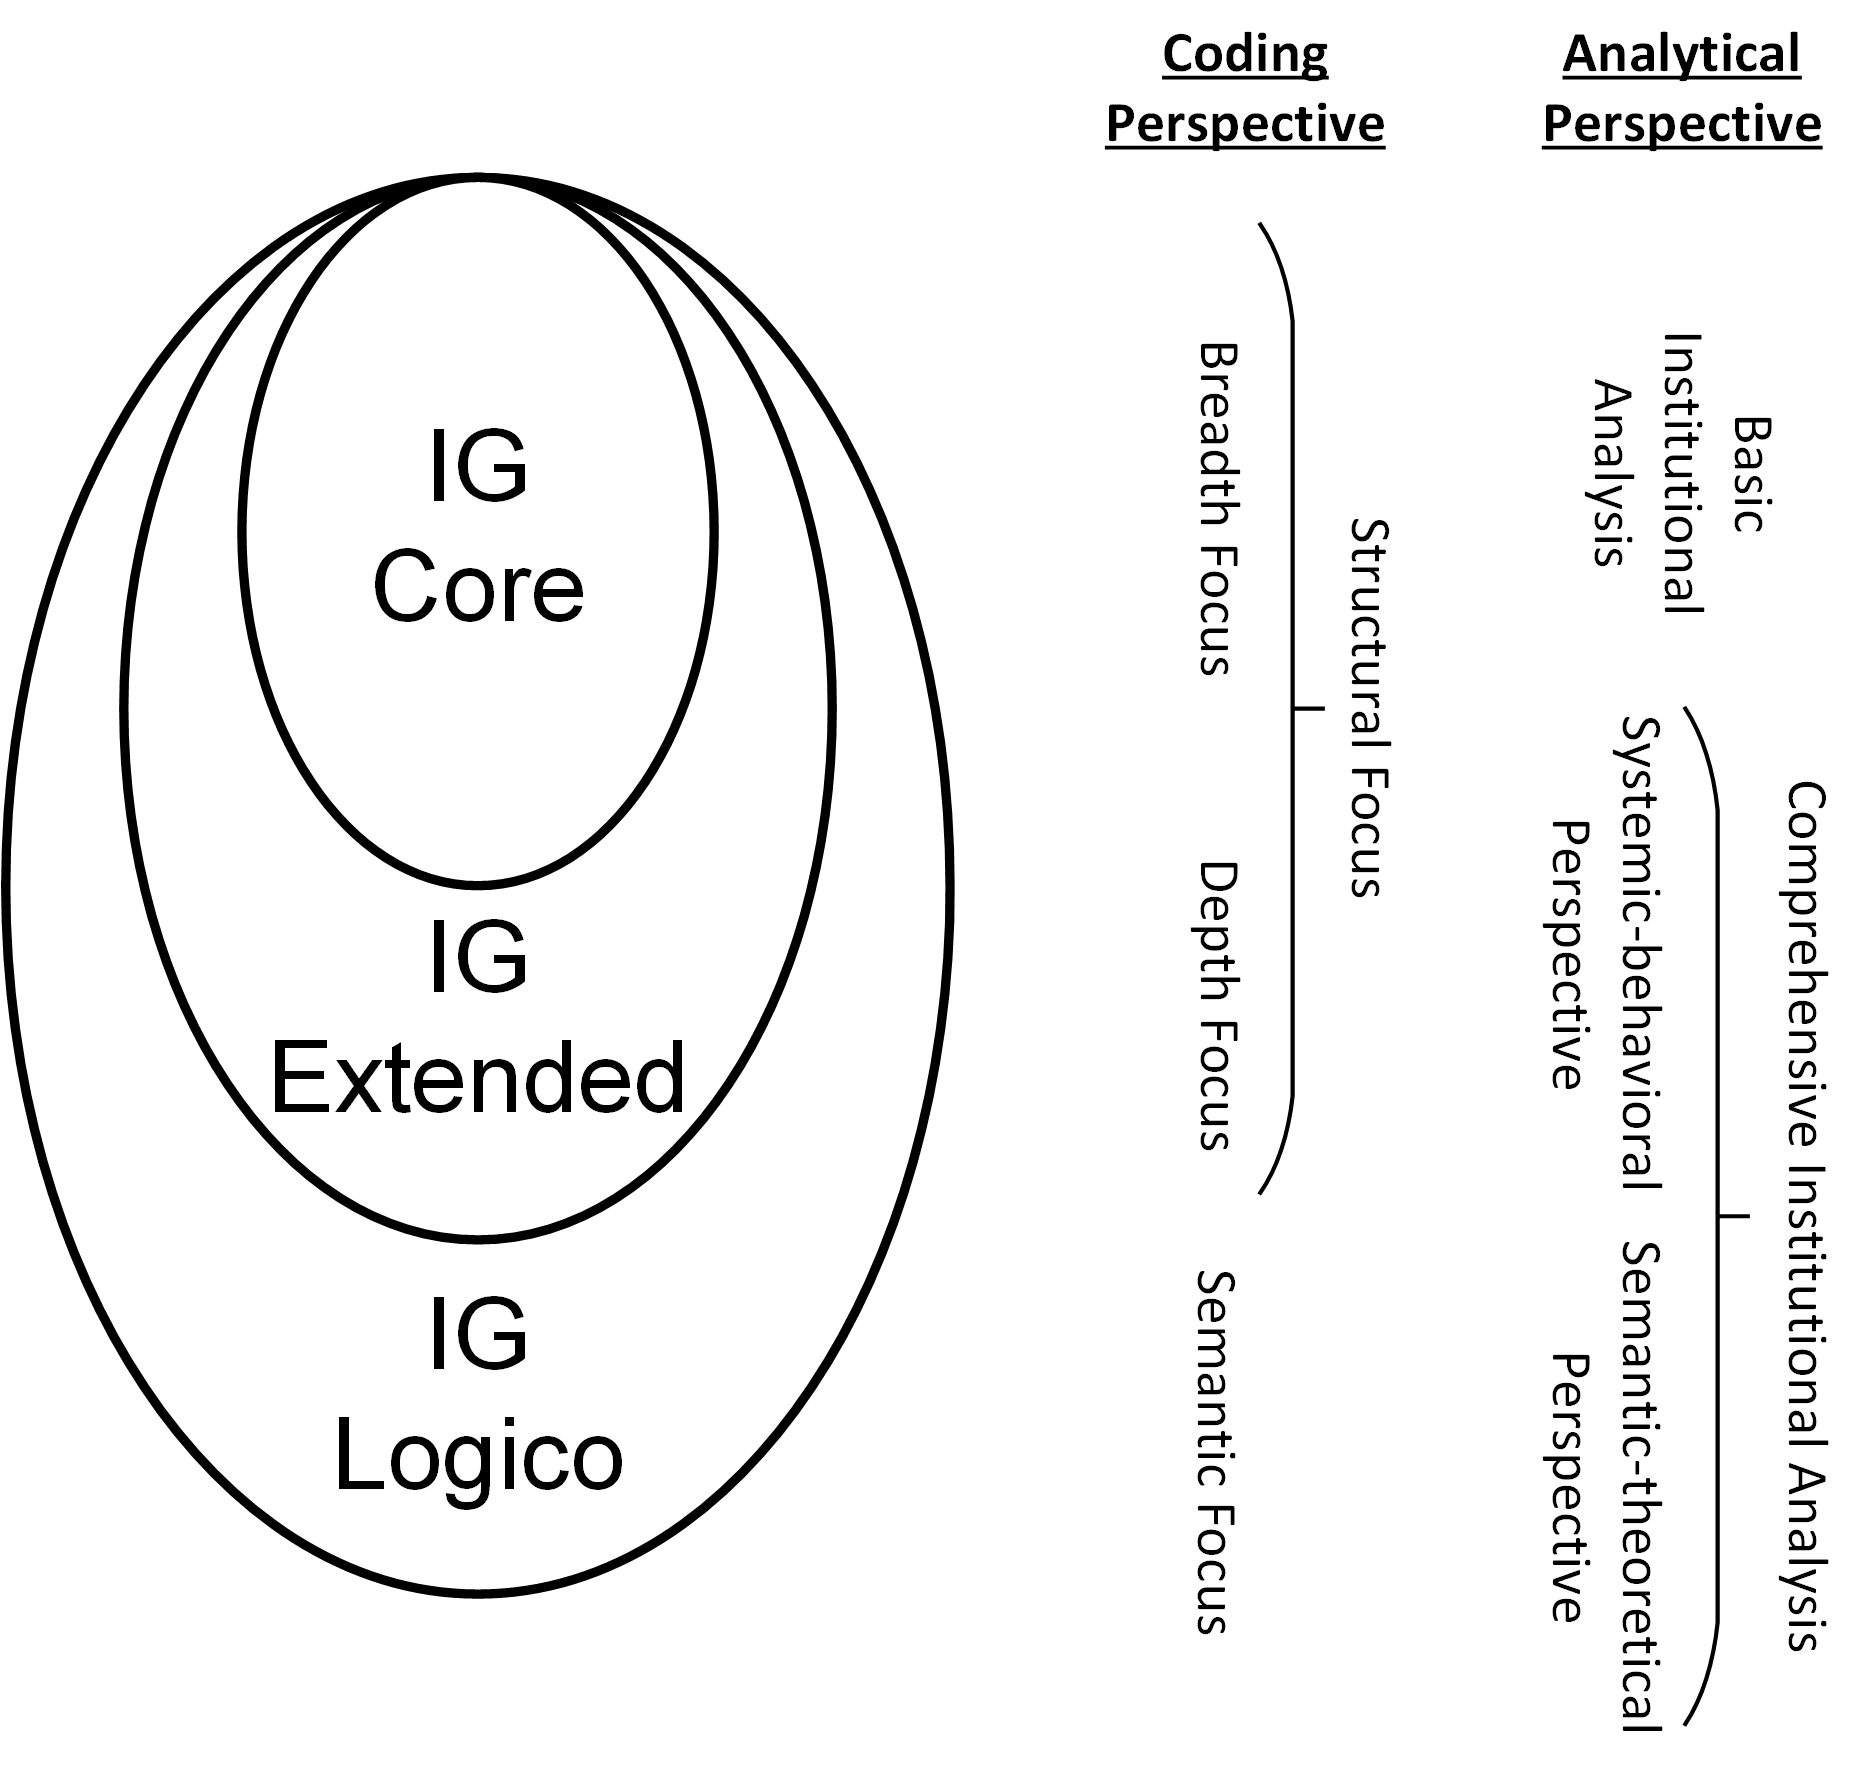
\includegraphics[width=0.5\textwidth]{figures/IGBibCoder.png}}
    \caption{Overview of IG Coding Levels and Associated Objectives}
    \label{fig:IgBibCoding}
\end{figure}

